% !TEX TS-program = pdflatex
% !TEX encoding = UTF-8 Unicode

% This is a simple template for a LaTeX document using the "article" class.
% See "book", "report", "letter" for other types of document.

\documentclass[11pt]{article} % use larger type; default would be 10pt

\usepackage{amsmath,amssymb}
\usepackage[utf8]{inputenc} % set input encoding (not needed with XeLaTeX)

%%% Examples of Article customizations
% These packages are optional, depending whether you want the features they provide.
% See the LaTeX Companion or other references for full information.

%%% PAGE 
\usepackage{geometry} % to change the page dimensions
\geometry{letterpaper} % or letterpaper (US) or a5paper or....
% \geometry{margin=2in} % for example, change the margins to 2 inches all round
% \geometry{landscape} % set up the page for landscape
%   read geometry.pdf for detailed page layout information
\usepackage{hyperref}
\usepackage{graphicx} % support the \includegraphics command and options

% \usepackage[parfill]{parskip} % Activate to begin paragraphs with an empty line rather than an indent

%%% PACKAGES
\usepackage{booktabs} % for much better looking tables
\usepackage{array} % for better arrays (eg matrices) in maths
\usepackage{paralist} % very flexible & customisable lists (eg. enumerate/itemize, etc.)
\usepackage{verbatim} % adds environment for commenting out blocks of text & for better verbatim
\usepackage{subfig} % make it possible to include more than one captioned figure/table in a single float
% These packages are all incorporated in the memoir class to one degree or another...

%%% HEADERS & FOOTERS
\usepackage{fancyhdr} % This should be set AFTER setting up the page geometry
\pagestyle{fancy} % options: empty , plain , fancy
\renewcommand{\headrulewidth}{0pt} % customise the layout...
\lhead{}\chead{}\rhead{}
\lfoot{}\cfoot{\thepage}\rfoot{}

%%% SECTION TITLE APPEARANCE
\usepackage{sectsty}
\allsectionsfont{\sffamily\mdseries\upshape} % (See the fntguide.pdf for font help)
% (This matches ConTeXt defaults)

%%% ToC (table of contents) APPEARANCE
\usepackage[nottoc,notlof,notlot]{tocbibind} % Put the bibliography in the ToC
\usepackage[titles,subfigure]{tocloft} % Alter the style of the Table of Contents

\usepackage{xcolor}

\renewcommand{\cftsecfont}{\rmfamily\mdseries\upshape}
\renewcommand{\cftsecpagefont}{\rmfamily\mdseries\upshape} % No bold!

\newcommand{\ns}[1]{\textcolor{red}{#1}}
%%% END Article customizations

%%% The "real" document content comes below...

\title{Consequences of Pauli blocking between paired fermions on Feshbach resonances}
%\author{The Author}
%\date{} % Activate to display a given date or no date (if empty),
         % otherwise the current date is printed 
\input{../newcommand}
\begin{document}
\maketitle
\section{Introduction}
Feshbach resonances plays an important role in the study of  phenomenon in dilute ultracold alkali gas, especially the BEC-BCS crossover phenomenon of the fermion gas. Feshbach resonances in the  two-body context was well understood \cite{Fano,nuclear, Leggett,ChinRMP}. When the bound-state level of a pair of  atomic hyperfine spins (subbands), (a.k.a. closed-channel), is closed to the threshold of the other pair of atomic hyperfine spins (subbands), (a.k.a open-channel),  the   effective attraction between two atoms in the open-channel are drastically modified.  This provides a unique tools for experimentalists to tune the effective interaction between two atoms via the magnetic field.    When we extend it into a many-body system, Pauli blocking needs to be taken into account for the identical fermionic atoms.  Roughly speaking, Pauli blocking manifests itself in two ways: First, within each channel, only at most one fermion pair can occupy each energy level;  Second, when two subbands share an atom of the the same hyperfine spin, only one channel can occupy the level of one specific momentum  $\vk$ level.

In the previous decade, one the authors (M. C.)  has developed a commutation theory of fermions pairs (composite bosons)\cite{CobosonPhysicsReports}.  This technique has been applied to various fields in the condensed matter physics with success.  Recently, this method has been applied to BCS theory \cite{combescotBCS,CobosonBcsRich}.  It works with another unique approach for the superconductivity by Richardson \cite{Richardson1, Richardson2, Richardson3} and Gaudin \cite{Gaudin} to convert the problem in a series of algebraic equations.  In the current report, this method is extended for the two-subband case to study the Feshbach resonance.  

The current report is organized as following: We first laid out the model in Sec. \ref{sec:model} and the commutation in Sec. \ref{sec:comm}.  We then proceed to study the one-pair, i.e. the two-body, problem in Sec. \ref{sec:one}. ....
\section{Model system \label{sec:model}}

We consider a system made of two different fermionic atoms, $\alpha$ and $\beta$.  These fermions can be in two coupled subbands. Let $\alpha^{\dg}_{\vk, \nu}$ and $\beta^{\dg}_{\vk,\nu}$, be the creation operators of fermions $\alpha$ and $\beta$ with momentum $\vk$ in one of these two subbands, $\nu=\pm1$. 

The Hamiltonian of this two-atom system reads as 
\begin{equation}\label{eq:H}
\mathcal{H}=\mathcal{H}_0+\mathcal{V}
\end{equation}
$\mathcal{H}_0$ is the free fermionic kinetic energy. 	
\begin{equation}
\mathcal{H}_0=\sum_{\nu=\pm1}\sum_{\vk}{(\epsilon_{\mathbf{k}}+\delta^{(\alpha)}_{\nu})\alpha^{\dg}_{\vk, \nu}\alpha^{}_{\vk, \nu}
+(\epsilon_{\mathbf{k}}+\delta^{(\beta)}_{\nu})\beta^{\dg}_{\vk, \nu}\beta^{}_{\vk, \nu}}				
\end{equation}	
where $\epsilon_{\mathbf{k}}=k^2/2m$ if these two atoms are taken with the same mass.  The lowest energy of the two $\alpha$ and $\beta$ subbands are $\eta_{\nu}^{(\alpha)}$ and 	 $\eta_{\nu}^{(\beta)}$ respectively. 

These $(\alpha,\beta)$ fermions are assumed to interact through a BCS-like separable potential having diagonal and non-diagonal processes.  This interaction potential, shown with Eq. \ref{eq:H}, can be written as 
\begin{equation}\label{eq:V}
\mathcal{V}=-\sum_{\{\nu\}}\sum_{\vk\vk{\prime}}w_{\vk}w_{\vk{\prime}}V 
\begin{pmatrix}
\nu_{\alpha}^{{\prime}}&\nu_{\alpha}^{}\\
\nu_{\beta}^{{\prime}}&\nu_{\beta}^{}
\end{pmatrix}
B^{\dg}_{\mathbf{k}^{{\prime}},\nu_{\alpha}^{{\prime}},\nu_{\beta}^{{\prime}}}
B^{}_{\mathbf{k}^{ },\nu_{\alpha}^{},\nu_{\beta}^{}}
\end{equation}
where, in order for $\mathcal{V}$ to be equal  $\mathcal{V}^{\dg}$, the $V 
\left(\begin{smallmatrix}
\nu_{\alpha}^{{\prime}}&\nu_{\alpha}^{}\\
\nu_{\beta}^{{\prime}}&\nu_{\beta}^{}
\end{smallmatrix}\right)$ prefactor is taken equal to $V 
\left(\begin{smallmatrix}
\nu_{\alpha}^{}&\nu_{\alpha}^{{\prime}}\\
\nu_{\beta}^{}&\nu_{\beta}^{{\prime}}
\end{smallmatrix}\right)$. 
$w_{\mathbf{k}}$ is a sharp cut-off function taken as identical for all interaction processes for simplicity. This cut-off allows us to get rid of spurious singularity.  The operator   $B^{\dg}_{\mathbf{k}^{ },\nu_{\alpha}^{},\nu_{\beta}^{}}$ creates an $(\alpha,\beta)$ pair with zero total momentum. The fermion $\alpha$ being in the subband $\nu_{\alpha}$ and the fermion $\beta$ in the subband $\nu_{\beta}$.  It reads 
\begin{equation}
B^{\dg}_{\mathbf{k}^{ },\nu_{\alpha}^{},\nu_{\beta}^{}}=a^{\dg}_{\mathbf{k}^{ },\nu_{\alpha}^{}}
b^{\dg}_{-\mathbf{k}^{ },\nu_{\beta}^{}}
\end{equation}
\begin{figure}[htbp]
\begin{center}
\includegraphics[width=0.6\textwidth]{VPair}
\caption{One pair interaction\label{fig:VPair}} 
%\parbox{0.7\textwidth}{\small }

\end{center}
\end{figure}


In order to study the effect of the Puli exclusion principle on paired fermions in coupled subbands, we are going to concentrate on two sets of interaction scatterings.  
\begin{enumerate}
\item The first set deals with pairs made of fermions, $\alpha$ and $\beta$, in different subbands, namely $P^{\dg}_{\vk,1,1}$ and $P^{\dg}_{\vk,-1,-1}$. These fermion pairs will then interact through the diagonal processes of Fig. \ref{fig:intra}, with a scattering called $v_{\eta}$, and through the non-diagonal process of Fig. \ref{fig:inter}, with a transfer scattering called $\tau$.  All the other $V 
\left(\begin{smallmatrix}\nu_{\alpha}^{{\prime}}&\nu_{\alpha}^{}\\ \nu_{\beta}^{{\prime}}&\nu_{\beta}^{}\end{smallmatrix}\right)$ scatterings are taken equal to zero.  When the number of fermions $\alpha$ and $\beta$ increases, the pairs $(\nu_{\alpha}=1, \nu_{\beta}=1)$ feel each other by Pauli blocking, as well as the pairs $(\nu_{\alpha}=-1, \nu_{\beta}=-1)$.
\begin{figure}[hhtb]
	\centering
	         \subfloat[Diagonal interaction]{\label{fig:intra}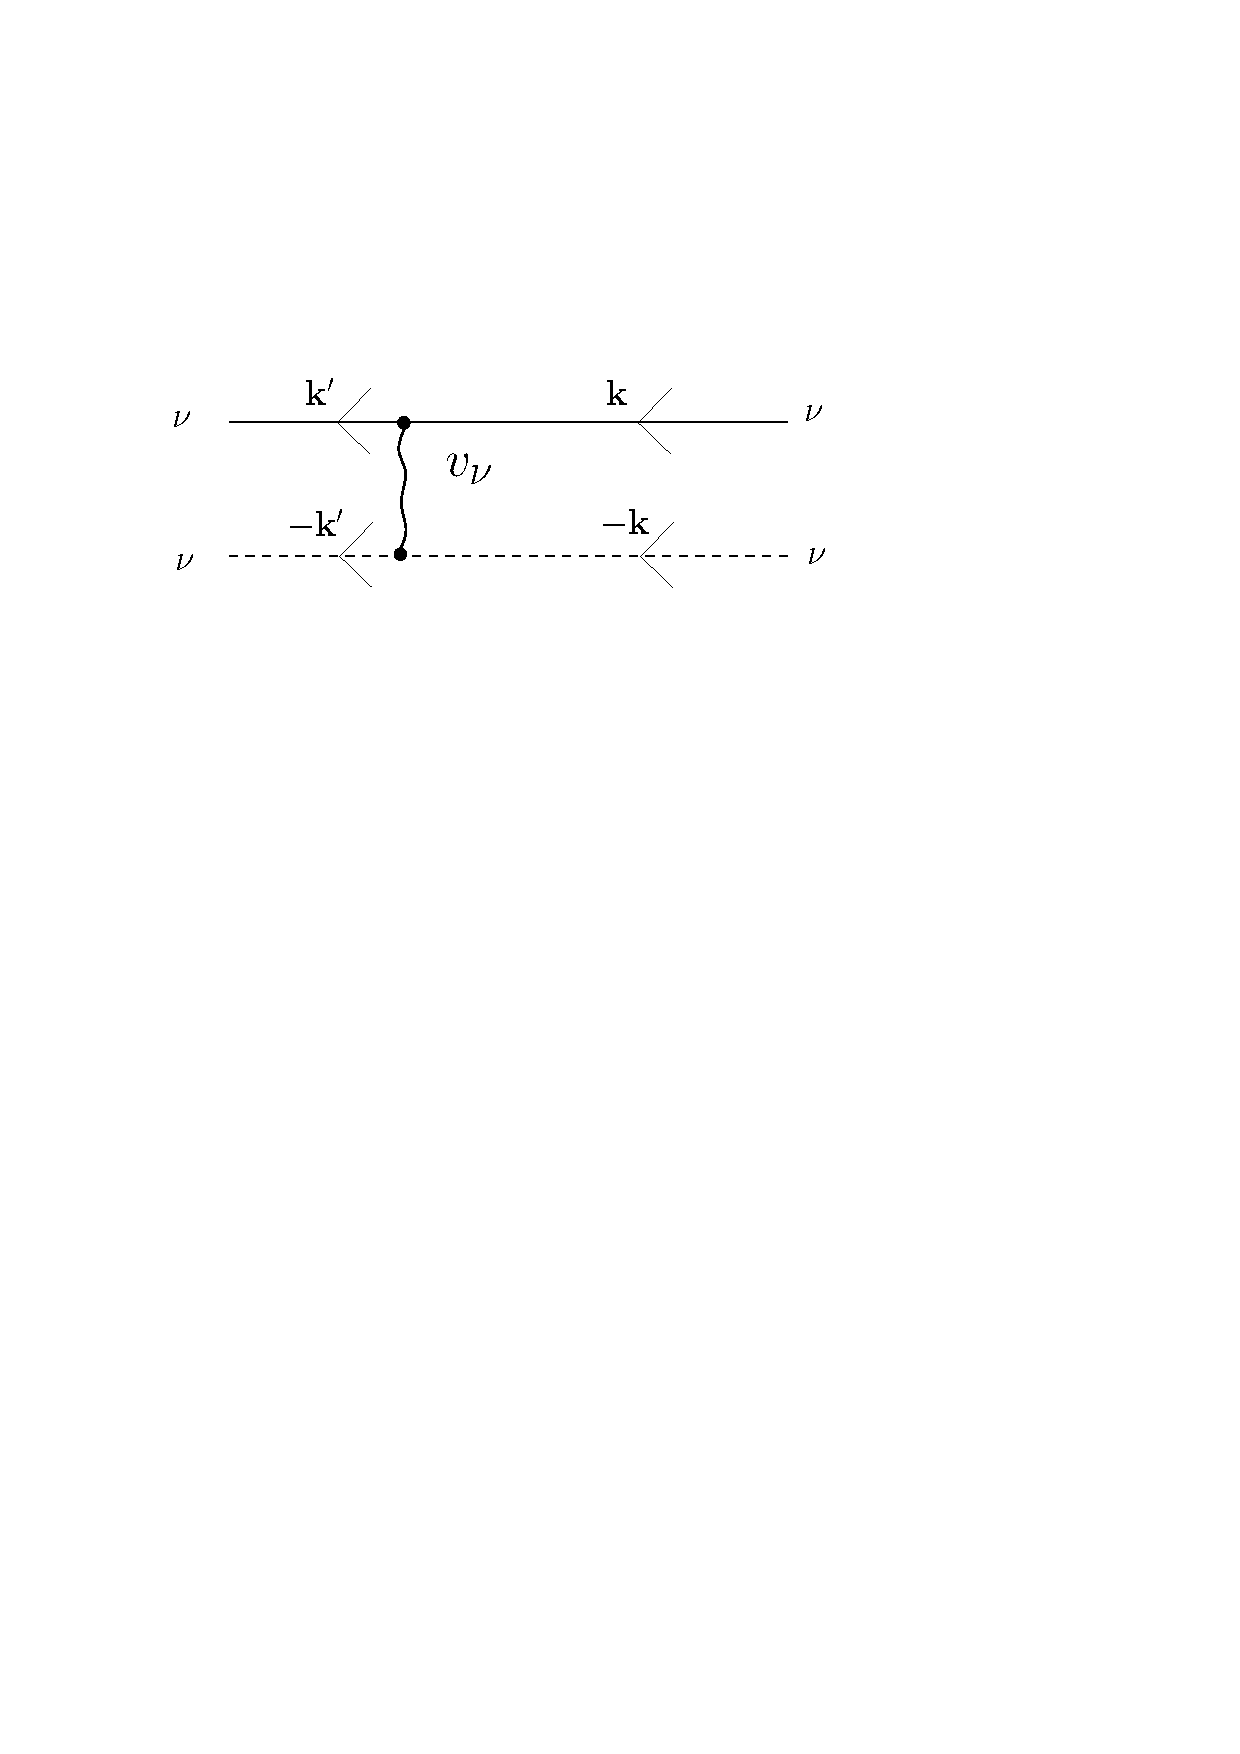
\includegraphics[width=.4\textwidth]{intraBand}}\qquad
		\subfloat[Non-diagonal interaction]{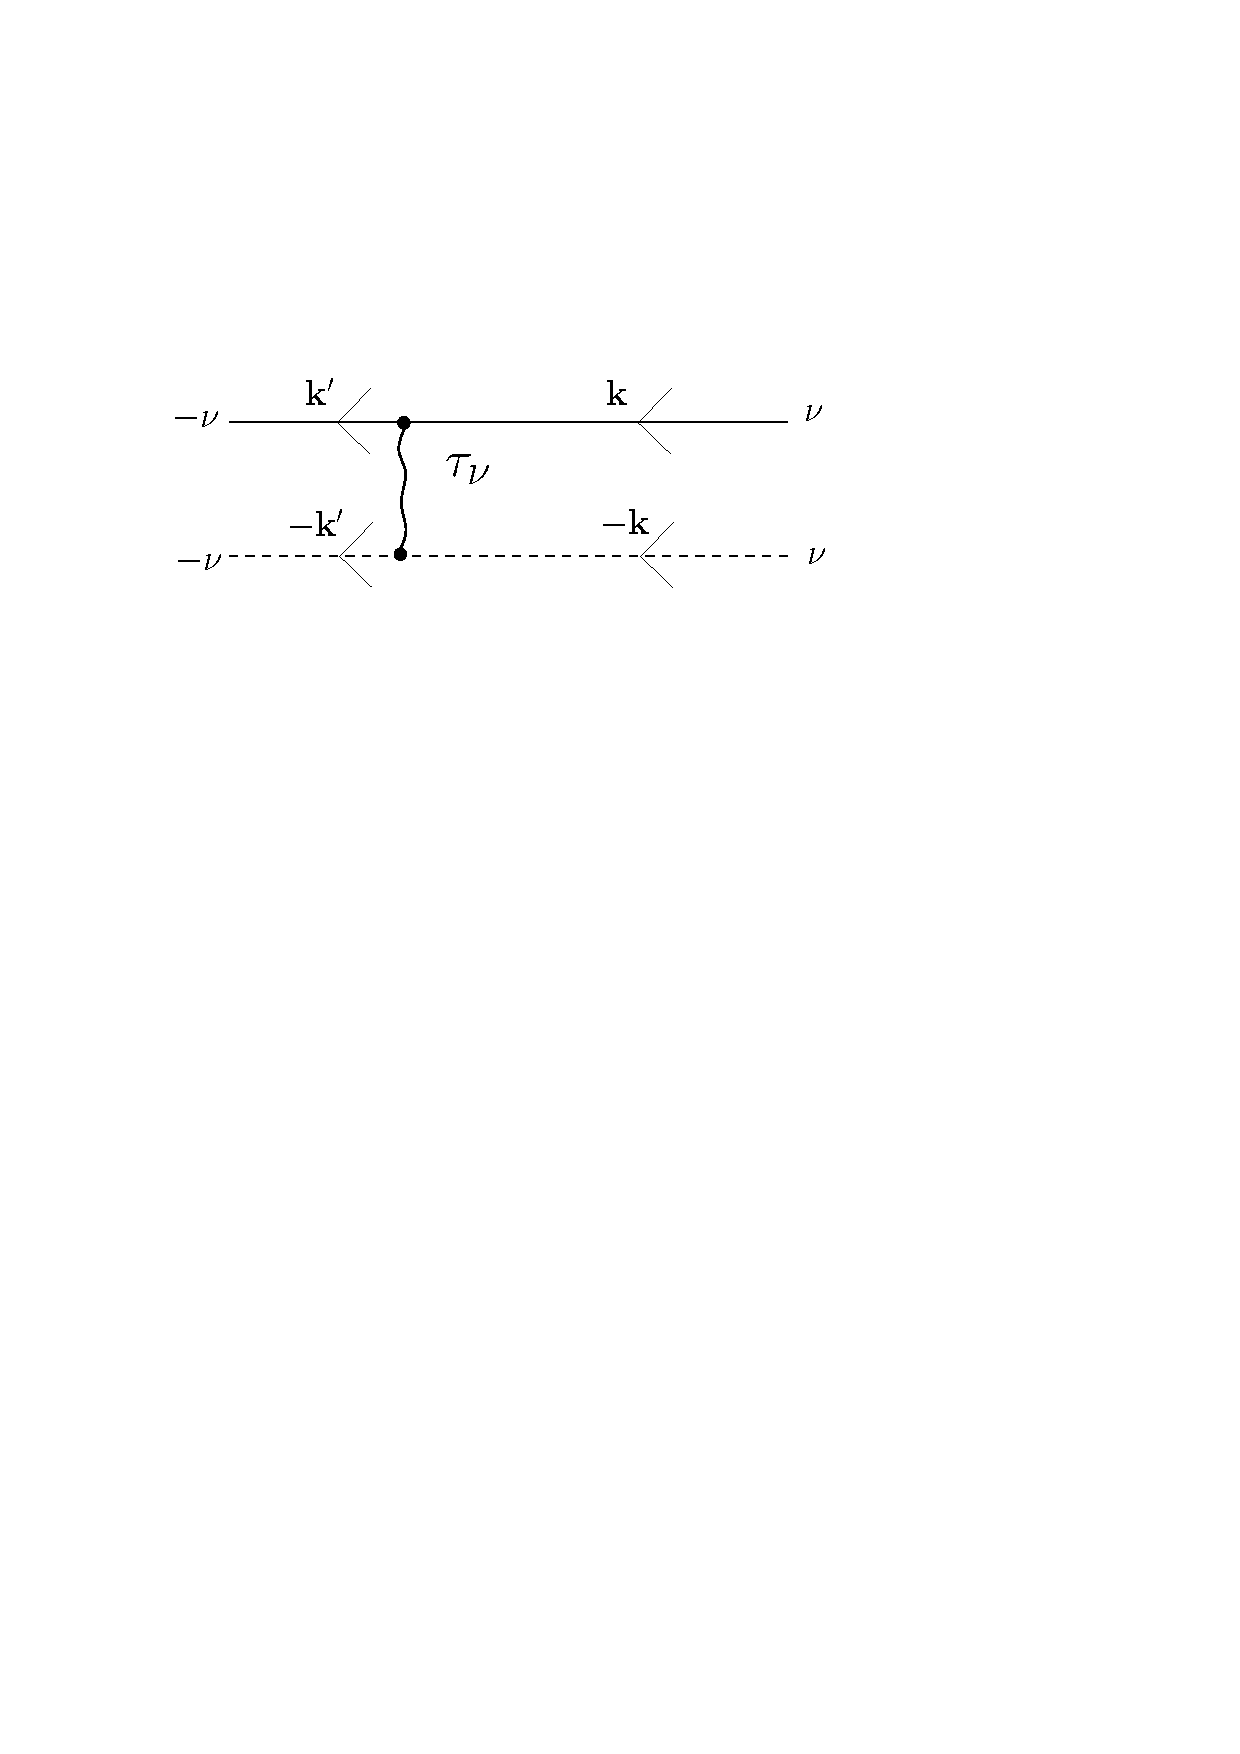
\includegraphics[width=.40\textwidth]{interBand}\label{fig:inter}}
	\caption{Diagonal and non-diagonal subband interaction without shared species}
\end{figure}
\item The second set of interaction potentials deals with pairs sharing a fermion $\alpha$ in subband $1$, namely $B^{\dg}_{\vk,1,1}$ and $B^{\dg}_{\vk,1,-1}$. These fermion pairs interact through the diagonal processes of Fig. \ref{fig:3intra}, with a scattering that we above call $v_{\eta}$ and through the transfer process of Fig. \ref{fig:3inter} with a transfer scattering $\tau$, the fermion $\alpha$ now staying in the $\nu=1$ band.  All the other $V 
\left(\begin{smallmatrix}\nu_{\alpha}^{{\prime}}&\nu_{\alpha}^{}\\ \nu_{\beta}^{{\prime}}&\nu_{\beta}^{}\end{smallmatrix}\right)$ scatterings are taken equal to zero.  In this case, the $(-1)$ states of fermion $\alpha$ stay uncoupled and play no role in the problem.  When the number of fermions $\alpha$ and $\beta$ increases, a $B^{\dg}_{\vk,1,1}$ pair feels not only the other $B^{\dg}_{\vk,1,1}$ pairs by Pauli blocking, but it also feels the $B^{\dg}_{\vk,1,-1}$ pairs because $B^{\dg}_{\vk,1,1}$ and $B^{\dg}_{\vk,1,-1}$ share the same fermion operator $a^{\dg}_{\vk,1}$.
\begin{figure}[hhtb]
	\centering
	         \subfloat[Diagonal interaction]{\label{fig:3intra}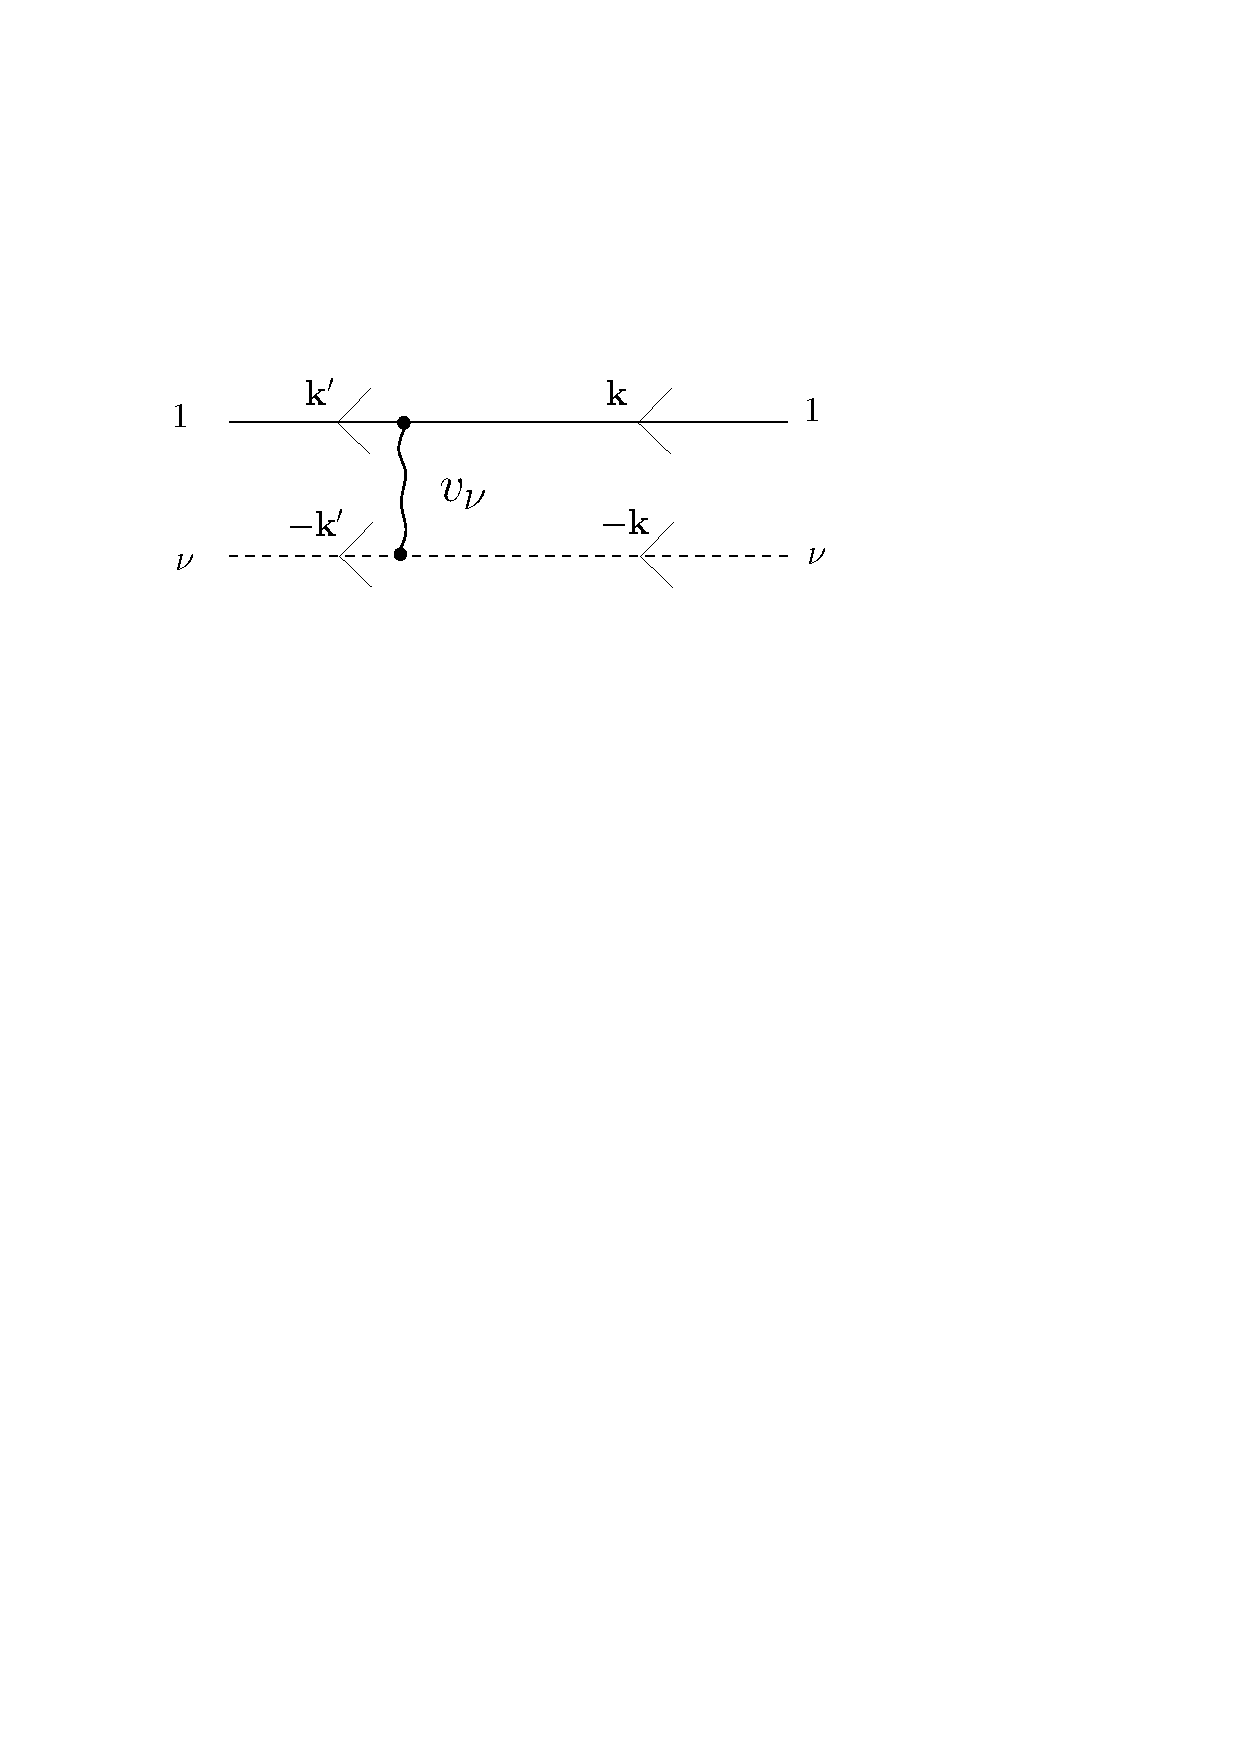
\includegraphics[width=.4\textwidth]{3intraBand}}\qquad
		\subfloat[Non-diagonal interaction]{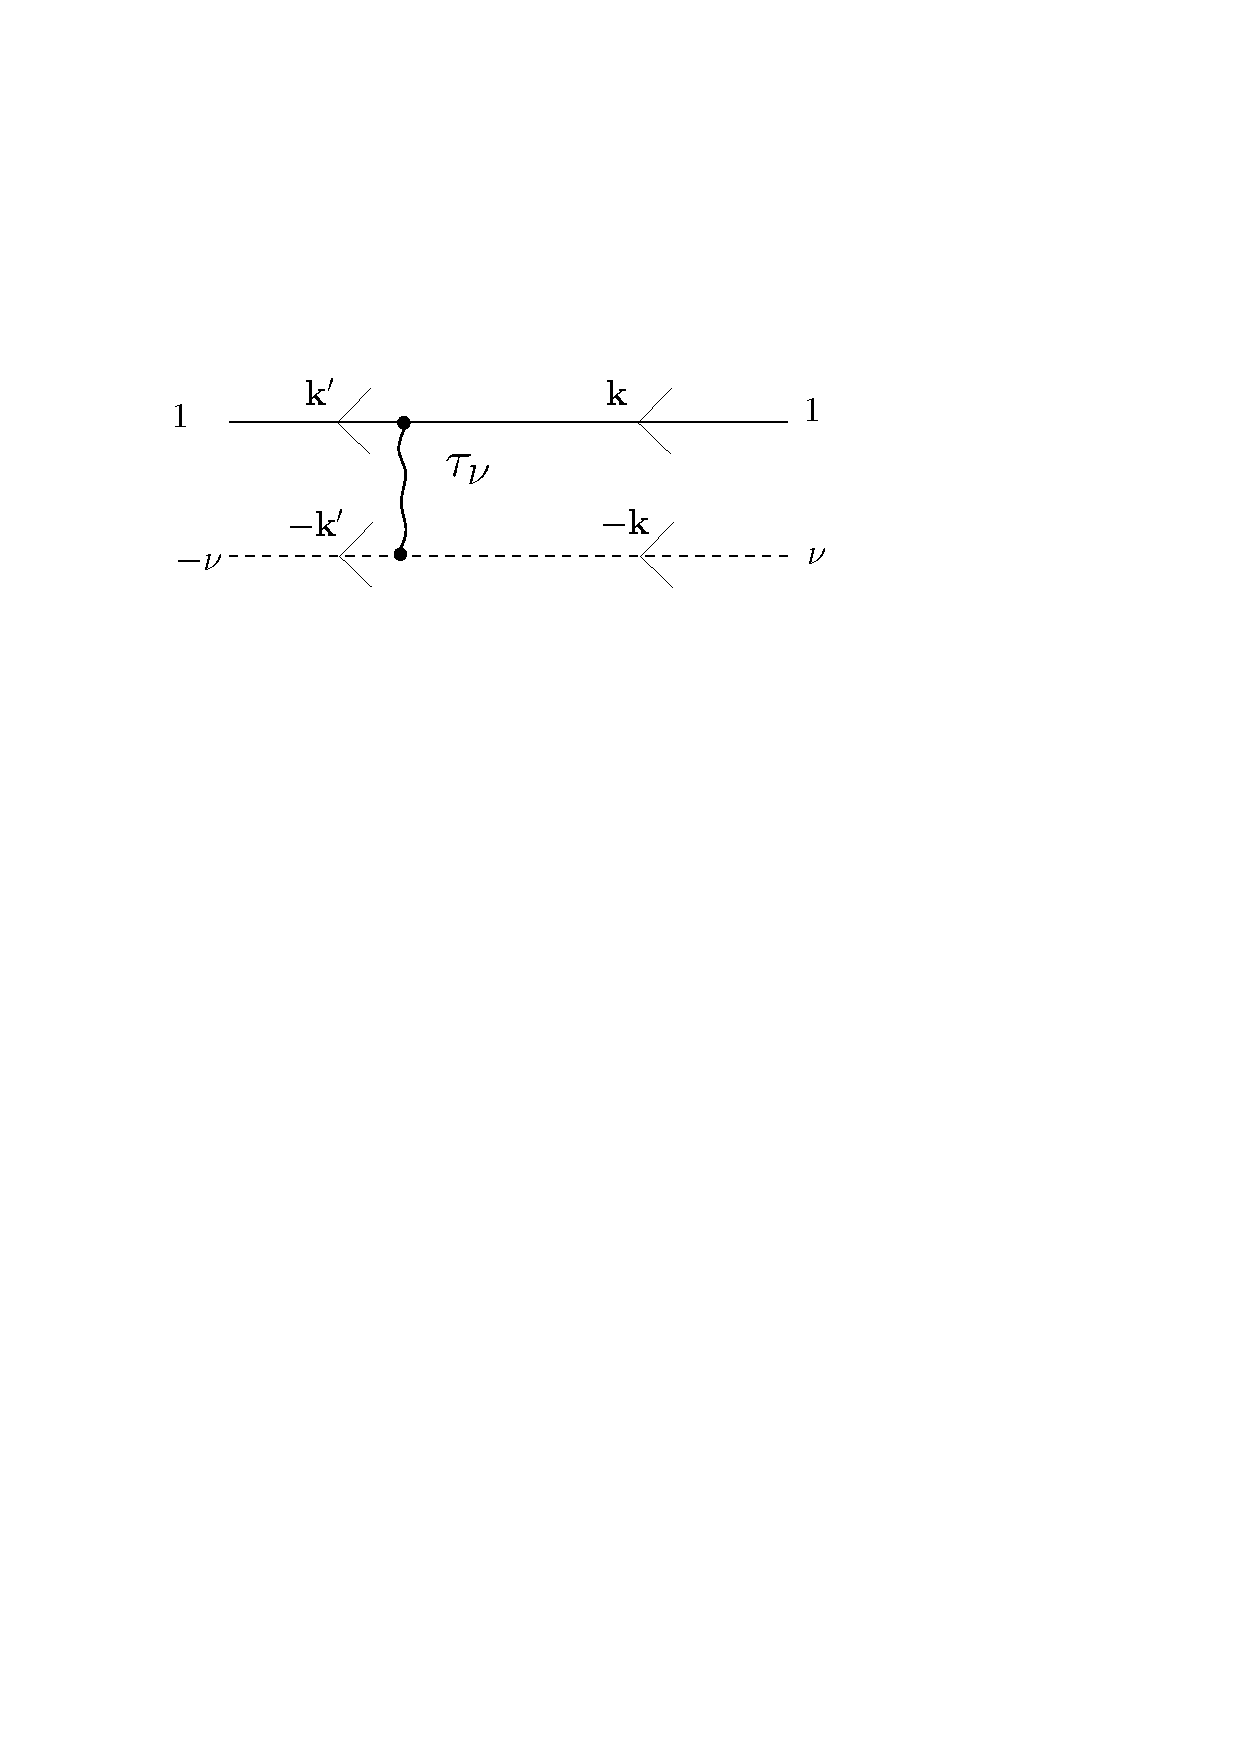
\includegraphics[width=.40\textwidth]{3interBand}\label{fig:3inter}}
	\caption{Diagonal and non-diagonal subband interaction with shared species}
\end{figure}
\end{enumerate}

Comparison between the results obtained within the two sets of interaction scatterings described above will help us to understand the very special role played by the Pauli exclusion principle in composite boson many-body effect, through differentiating Pauli blocking between a given set of pairs $B^{\dg}_{\vk,\eta,\eta}$ and between different sets of pairs $B^{\dg}_{\vk,\eta,\eta}$ and $B^{\dg}_{\vk,\eta,-\eta}$.

Feshbach resonances provide a very unique tool to test this understanding. Indeed, by changing the magnetic field felt by the $(\alpha,\beta)$ atoms, we can change the subband energy differences $\eta^{(\alpha)}=\eta^{(\alpha)}_1-\eta^{(\alpha)}_{-1}$ and  $\eta^{(\beta)}=\eta^{(\beta)}_1-\eta^{(\beta)}_{-1}$ without substantially changing the potential scattering $v_{\eta}$ and $\tau$.  In the absence of subband {transfer}, $\tau=0$, a pair of fermions $(\alpha,\beta)$ in subband $1$ can have a bound state if $v_1$ is large enough.  By changing the magnetic field, the pair energy of this bound state, $\eta^{(\alpha)}_1+\eta^{(\beta)}_{1}-\epsilon_1^*$ when $\epsilon_1^*$ is the bound state binding energy, can cross the energy  $\eta^{(\alpha)}_{-1}+\eta^{(\beta)}_{-1}$ or  $\eta^{(\alpha)}_{1}+\eta^{(\beta)}_{-1}$ of a fermion pair in the $(-1)$ subband, ``open channel", i.e., when the $v_{-1}$ potential is too small to bind a  $(\alpha,\beta)$ pair. The goal of the present work is to describe this anticrossing in the presence of a finite potential $\tau$.  If we only have one fermion pair  $(\alpha,\beta)$, the problem is  rather simple to the single Cooper pair problem and the exact analytical result is easy to extend to finite $\tau$.  The interesting question raised by Pauli blocking between fermion pairs sharing a common fermion, \ns{case} when the number of pairs gets larger than $1$.  The energy of two Cooper pairs with Pauli blocking between them treated exactly has recently been bound in the absence of coupling $\tau$\cite{combescotBCS}.  Its extension to finite $\tau$ {yet} is quite valuable as it indicates the trend induced by the Pauli exclusion principle on the single pair solution.  As already shown in the absence of transfer, $\tau=0$, this trend is of great help to physically understand what the Pauli exclusion really does in the far more complex case of $N$ pairs and more generally along the BEC-BCS crossover in a two channel configuration. 

\section{Commutation relations\label{sec:comm}}
A nice way to handle the Pauli exclusion principle between paired fermions is through a commutation formalism similar to the one we developed for semiconductor excitons\cite{CobosonPhysicsReports}.  Let us first derive a few commutators useful in the present problem. 

For fermion operators $a^{\dg}_{\vk\nu_{\alpha}}$ and $b^{\dg}_{\vk\nu_{\beta}}$ having standard anticommuation relations, we easily get the following commutators
\begin{equation}
[B^{\dg}_{\mathbf{k}^{{\prime}},\nu_{\alpha}^{{\prime}},\nu_{\beta}^{{\prime}}},B^{\dg}_{\mathbf{k}^{ },\nu_{\alpha}^{},\nu_{\beta}^{}}]=0
\end{equation}
\begin{equation}\label{eq:bb}
[B^{}_{\mathbf{k}^{\prime },\nu_{\alpha}^{{\prime}},\nu_{\beta}^{{\prime}}},B^{\dg}_{\mathbf{k}^{ },\nu_{\alpha}^{},\nu_{\beta}^{}}]=
	\delta_{\mathbf{k}^{ },\mathbf{k}^{{\prime}}}\delta_{\nu_{\alpha}^{},\nu_{\alpha}^{{\prime}}}\delta_{\nu_{\beta}^{},\nu_{\beta}^{{\prime}}}-
	D^{}_{\mathbf{k}^{{\prime} },\nu_{\alpha}^{{\prime}},\nu_{\beta}^{{\prime}};\,\mathbf{k}^{ },\nu_{\alpha}^{},\nu_{\beta}^{}}
\end{equation}
The operator $D^{}_{\mathbf{k}^{{\prime} },\nu_{\alpha}^{{\prime}},\nu_{\beta}^{{\prime}};\,\mathbf{k}^{ },\nu_{\alpha}^{},\nu_{\beta}^{}}$ is precisely given by
\begin{equation}
D^{}_{\mathbf{k}^{{\prime} },\nu_{\alpha}^{{\prime}},\nu_{\beta}^{{\prime}};\,\mathbf{k}^{ },\nu_{\alpha}^{},\nu_{\beta}^{}}=
	\delta_{\mathbf{k}^{ },\mathbf{k}^{{\prime}}}(\delta_{\nu_{\alpha}^{},\nu_{\alpha}^{{\prime}}}b^{\dg}_{-\vk\nu_{\beta}}b^{}_{-\vk\nu_{\beta}^{{\prime}}}+\delta_{\nu_{\beta}^{},\nu_{\beta}^{{\prime}}}a^{\dg}_{\vk\nu_{\alpha}^{}}a^{}_{\vk\nu_{\alpha}^{{\prime}}})
\end{equation}
comes from the composite boson nature of fermion pairs.  This operator gives zero when acting on a vacuum while its effect on other paired electrons follows from 

\begin{equation}\label{eq:db}
\big[D^{}_{\mathbf{k}^{{\prime}{\prime} },\nu_{\alpha}^{{\prime}{\prime}},\nu_{\beta}^{{\prime}{\prime}};\mathbf{k}^{{\prime} },\nu_{\alpha}^{{\prime}},\nu_{\beta}^{{\prime}}},\,B^{\dg}_{\mathbf{k}^{ },\nu_{\alpha}^{},\nu_{\beta}^{}}\big]=
	\delta_{\mathbf{k}^{ },\mathbf{k}^{{\prime}}}\delta_{\mathbf{k}^{{\prime}{\prime} },\mathbf{k}^{{\prime}}}
	\Big(\delta_{\nu_{\alpha}^{{\prime}{\prime}},\nu_{\alpha}^{{\prime}}}\delta_{\nu_{\beta}^{{\prime}{\prime}},\nu_{\beta}^{}}B^{\dg}_{\mathbf{k}^{ },\nu_{\alpha}^{},\nu_{\beta}^{{\prime}}}+
	\delta_{\nu_{\alpha}^{{\prime}{\prime}},\nu_{\alpha}^{}}\delta_{\nu_{\beta}^{{\prime}{\prime}},\nu_{\beta}^{{\prime}}}B^{\dg}_{\mathbf{k}^{ },\nu_{\alpha}^{{\prime}},\nu_{\beta}^{}}\Big)
\end{equation}
Using these commutators, it is easy to find the effects o f the potential $\mathcal{V}$ defined in Eq. \ref{eq:V} on paired electrons while the free part $\mathcal{H}_0$ of the Hamiltonian follows from
\begin{equation}\label{eq:h0B}
\big[H_0,\,B^{\dg}_{\mathbf{k}^{ },\nu_{\alpha}^{},\nu_{\beta}^{}}\big]=
	(2\epsilon_{\vk}+\epsilon_{\nu_{\alpha}\nu_{\beta}})B^{\dg}_{\mathbf{k}^{ },\nu_{\alpha}^{},\nu_{\beta}^{}}
\end{equation}
where 
\begin{equation}
\epsilon_{\nu_{\alpha}\nu_{\beta}}=\eta_{\nu_{\alpha}}^{(\alpha)}+\eta_{\nu_{\beta}}^{(\beta)}
\end{equation}
We now use these commutators to calculate the ground state energy of one and two pairs of fermions $\alpha$ and $\beta$ in the two relevant configurations, namely, when this ground state is made of $(B^{\dg}_{\mathbf{k}^{ },1,1}, B^{\dg}_{\mathbf{k}^{ },-1,-1})$ pairs and when it is made of $(B^{\dg}_{\mathbf{k}^{ },1,1}, B^{\dg}_{\mathbf{k}^{ },1,-1})$ pairs. We expect to see some difference when the fact, that these pairs share a common fermion, plays a role through Pauli blocking.  This is going to happen for more than one fermion pairs.  A new Pauli blocking channel then opens, {compared} to the one which already exists when the number of composite bosons goes from $1$ to $2$.  For a deep understanding of these two channels, let us first show that one-fermion pair ground state carefully when a transfer between subbands $1$ and $-1$ exists. 

\section{One-pair ground state\label{sec:one}}
\subsection{ Pairs made of $(B^{\dg}_{\mathbf{k}^{ },1,1}$ and $B^{\dg}_{\mathbf{k}^{ },-1,-1})$}

The relevant part of the interaction potential $\mathcal{V}$ defined in Eq. \ref{eq:V} then reduced to $V+T$. The diagonal part is given by 
\begin{equation}\label{eq:V}
V=-\sum_{\nu=\pm1}v_{\nu}\sum_{\vk,\vk^{{\prime}}}
w_{\vk}w_{\vk{\prime}}
B^{\dg}_{\mathbf{k}^{{\prime}},\nu,\nu}
B^{}_{\mathbf{k}^{ },\nu,\nu}
\end{equation}
and the transfer part 
\begin{equation}\label{eq:T}
T=-\tau\sum_{\nu=\pm1}\sum_{\vk,\vk^{{\prime}}}
w_{\vk}w_{\vk{\prime}}
B^{\dg}_{\mathbf{k}^{{\prime}},-\nu,-\nu}
B^{}_{\mathbf{k}^{ },\nu,\nu}
\end{equation}

Using Eq. \ref{eq:h0B}, we find
\begin{equation}
H_0\,B^{\dg}_{\mathbf{k}^{ },\nu,\nu}|0\rangle=
\big[H_0,\,B^{\dg}_{\mathbf{k}^{ },\nu,\nu}\big]|0\rangle=
(2\epsilon_{\vk}+\eta_{\nu}^{(\alpha)}+\eta_{\nu}^{(\beta)})B^{\dg}_{\mathbf{k}^{ },\nu,\nu}|0\rangle
\end{equation}
Eq. \ref{eq:bb} and the fact that the operator $D^{}_{\mathbf{k}^{{\prime}{\prime} },\nu_{\alpha}^{{\prime}{\prime}},\nu_{\beta}^{{\prime}{\prime}};\mathbf{k}^{{\prime} },\nu_{\alpha}^{{\prime}},\nu_{\beta}^{{\prime}}}$ gives zero on vacuum, allows us to write the diagonal part $V$ acting on one pair as 
\begin{equation}
VB^{\dg}_{\mathbf{k}^{ },\nu,\nu}|0\rangle=-\sum_{\nu^{{\prime}}}v_{\nu^{{\prime}}}\sum_{\vp^{{\prime}}vp^{}}w_{\vp^{{\prime}}}w_{\vp}B^{\dg}_{\mathbf{p}^{ },\nu^{{\prime}},\nu^{{\prime}}}[B^{}_{\mathbf{p}^{ },\nu^{{\prime}},\nu^{{\prime}}},B^{\dg}_{\mathbf{k}^{ },\nu,\nu}]|0\rangle=-v_{\nu}w_{\vk}\beta^{\dg}_{\nu,\nu}
\end{equation}
where we have set
\begin{equation}\label{eq:beta}
\beta^{\dg}_{\nu,\nu}=\sum_{\vp^{{\prime}}}B^{\dg}_{\mathbf{p}^{{\prime}},\nu,\nu}
\end{equation}
In the same way, the transient part of the potential gives
\begin{equation}
TB^{\dg}_{\mathbf{k}^{ },\nu,\nu}|0\rangle=-\tau{}w_{\vk}\beta^{\dg}_{-\nu,-\nu}
\end{equation}

We now look for the one-pair expectation of $\mathcal{H}_0+V+T$ as 
\begin{equation}\label{eq:Psi1}
|\Psi_1\rangle=\sum_{\nu=\pm1}\sum_{\vk}\phi_{\vk,\nu}B^{\dg}_{\mathbf{k}^{ },\nu,\nu}|0\rangle
\end{equation}
The above equations allow us to write the Schr\"odinger equation for one-pair $0=(\mathcal{H}_0+V+T)|\Psi_1\rangle$ as 
\begin{equation}
\begin{split}
0=&\sum_{\nu\vk}(2\epsilon_{\vk}+\eta_{\nu_{\alpha}}^{(\alpha)}+\eta_{\nu_{\beta}}^{(\beta)}-E_1)\phi_{\vk\nu}B^{\dg}_{\mathbf{k}^{ },\nu,\nu}\\
&-\sum_{\nu\vk}w_{\vk}\phi_{\vk,\nu}v_{\nu}\sum_{\vp}w_{\vp}B^{\dg}_{\mathbf{p}^{ },\nu,\nu}
 -\tau\sum_{\nu\vk}w_{\vk}\phi_{\vk,\nu}\sum_{\vp}w_{\vp}B^{\dg}_{\mathbf{p}^{ },-\nu,-\nu}
\end{split}
\end{equation}
By changing $\nu$ to $-\nu$ in the last term, we can rewrite this equation in a compact form as 
\begin{equation}\label{eq:schOne}
\begin{split}
0=&\sum_{\nu\vk}B^{\dg}_{\mathbf{k}^{ },\nu,\nu}\Big\{(2\epsilon_{\vk}+\eta_{\nu_{\alpha}}^{(\alpha)}+\eta_{\nu_{\beta}}^{(\beta)}-E_1)\phi_{\vk\nu}\\
&\quad-w_{\vk}v_{\nu}\sum_{\vp}w_{\vp}\phi_{\vp,\nu}-\tau{}w_{\vk}\sum_{\vp}w_{\vp}\phi_{\vp,-\nu}\Big\}|0\rangle
\end{split}
\end{equation}
This equation imposes the prefactor to be zero. 

(i) For $v_{\nu}=0=\tau$, the solution is $2\epsilon_{\vk}+\eta_{\nu_{\alpha}}^{(\alpha)}+\eta_{\nu_{\beta}}^{(\beta)}=E_1$, i.e. $\phi_{\vk^{{\prime}}\nu}=0$ for $\vk^{{\prime}}\neq\vk$ while $\phi_{\vk^{{\prime}}\nu}$ can differ from zero for  $\vk^{{\prime}}\neq\vk$. This result just corresponds to free fermion pairs in two uncoupled subbands, as expected. 

For $v_{\nu}$ or $\tau$ different from zero, the solution of Eq. \ref{eq:schOne} reads
\begin{equation}\label{eq:phi}
\phi_{\vk^{}\nu}=\Big(v_{\nu}\sum_{\vp}w_{\vp}\phi_{\vp,\nu}+\tau{}\sum_{\vp}w_{\vp}\phi_{\vp,-\nu}\Big)
\frac{w_{\vk}}{2\epsilon_{\vk}+\eta_{\nu_{\alpha}}^{(\alpha)}+\eta_{\nu_{\beta}}^{(\beta)}-E_1}
\end{equation}
To get the equation fullfilled by the energy, we multiply the above equation by $w_{\vk}$ and we sum over $\vk$.  This gives 
\begin{equation}\label{eq:phiS}
\sum_{\vk}w_{\vk}\phi_{\vk^{}\nu}=\Big(v_{\nu}\sum_{\vp}w_{\vp}\phi_{\vp,\nu}+\tau{}\sum_{\vp}w_{\vp}\phi_{\vp,-\nu}\Big)
S(E_1-\eta_{\nu_{\alpha}}^{(\alpha)}-\eta_{\nu_{\beta}}^{(\beta)})
\end{equation}
where we have 
\begin{equation}\label{eq:Sdef}
S(E)=\sum_{\vk}\frac{w_{\vk}}{2\epsilon_{\vk}-E}
\end{equation}

This gives two homogeneous equations for $\sum_{\vk}w_{\vk}\phi_{\vk\nu}$ with $\nu=\pm1$. They read
\begin{equation}\label{eq:tauEq}
[1-v_{\nu}S(E_1-\eta_{\nu_{\alpha}}^{(\alpha)}-\eta_{\nu_{\beta}}^{(\beta)})]\sum_{\vk}w_{\vk}\phi_{\vk^{}\nu}
=\tau{}S(E_1-\eta_{\nu_{\alpha}}^{(\alpha)}-\eta_{\nu_{\beta}}^{(\beta)})\sum_{\vk}w_{\vk}\phi_{\vk^{}-\nu}
\end{equation}
These equations have a non-zero solution provided that their determent is equal to zero.  This gives the one-pair eigenstate through an algebraic  equation which reads as 
\begin{multline}
[1-v_{1}S(E_1-\eta_{1}^{(\alpha)}-\eta_{1}^{(\beta)})][1-v_{-1}S(E_1-\eta_{-1}^{(\alpha)}-\eta_{-1}^{(\beta)})]\\
=\tau^2S(E_1-\eta_{1}^{(\alpha)}-\eta_{1}^{(\beta)})S(E_1-\eta_{-1}^{(\alpha)}-\eta_{-1}^{(\beta)})\label{eq:tauEq2}
\end{multline}
Using Eq. \ref{eq:phi}, we get the one-pair eigenstate given in Eq. \ref{eq:Psi1} as
\begin{equation}
|\Psi_1\rangle=\sum_{\nu=\pm1}\Big(v_{\nu}\sum_{\vp}w_{\vp}\phi_{\vp,\nu}+\tau{}\sum_{\vp}w_{\vp}\phi_{\vp,-\nu}\Big)B^{\dg}_{\nu,\nu}(E_{1})|0\rangle
\end{equation}
where $B^{\dg}_{\nu,\nu}(E_{1})|0\rangle=\sum_{\vk}\frac{w_{\vk}}{2\epsilon_{\vk}+\eta_{\nu_{\alpha}}^{(\alpha)}+\eta_{\nu_{\beta}}^{(\beta)}-E_1}\beta^{\dg}_{\nu,\nu}|0\rangle$ by Cooper, namely Eq. \ref{eq:phiS} allows us to rewrite this equation as 
\begin{equation}
|\Psi_1\rangle=\sum_{\nu=\pm1}\frac{\sum_{\vp}w_{\vp}\phi_{\vp\nu}}{S(E_1-\eta_{\nu_{}}^{(\alpha)}-\eta_{\nu_{}}^{(\beta)})}B^{\dg}_{\nu,\nu}(E_{1})|0\rangle
\end{equation}
It is actually possible to transform this symmetrical expression in $\nu=\pm1$ in order to have the transfer coupling $\tau$ appearing \ns{effectively} in $|\Psi_1\rangle$.  To do it, we rewrite the $\sum_{\vp}w_{\vp}\phi_{\vp\nu}$ sum according to Eq. \ref{eq:tauEq} taken for $\nu=-1$.  We then first write an {irrelevant} prefector $\frac{\sum_{\vp}w_{\vp}\phi_{\vp\nu}}{S(E_1-\eta_{\nu_{}}^{(\alpha)}-\eta_{\nu_{}}^{(\beta)})}$ that $|\Psi_1\rangle$ also reads
\begin{equation}\label{eq:Psi1B}
|\Psi_1\rangle=B^{\dg}_{1,1}(E_{1})|0\rangle+X_{1,-1}B^{\dg}_{-1,-1}(E_{1})|0\rangle
\end{equation}
$X_{1,-1}$ describes the subband mixing introduced by the potential transfer $\tau$.  It precisely reads
\begin{equation}
X_{1,-1}=\frac{\tau{}S(E_1-\eta_{1}^{(\alpha)}-\eta_{1}^{(\beta)})}{1-v_{\nu}S(E_1-\eta_{-1}^{(\alpha)}-\eta_{-1}^{(\beta)})}
\end{equation}
Eqs. (\ref{eq:tauEq2}, \ref{eq:Psi1B}) readily shows that, as expected, the one-pair eigenstates reduce, in the absence of transfer $\tau=0$, to the one-pair eigenstate obtained by Cooper, the pairs being made of fermions $\alpha$ and $\beta$ which either belong to the subbands $1$ with energy $\eta^{(\alpha)}_{1}+\eta^{(\beta)}_{1}$ or to the subband $-1$ with energy $\eta^{(\alpha)}_{-1}+\eta^{(\beta)}_{-1}$.  For finite transfer $\tau$,  these two independent  pair solutions which the two independent pair solutions which are moreover taken for slightly different energy $E_{1}$ if $\tau$ is small. 

\subsection{Pairs made of $B^{\dg}_{\vk,1,1}$ and $B^{\dg}_{\vk,1,-1}$}
We now consider $(\alpha,\beta)$ pairs sharing their fermion $\alpha$, this fermion being in the $\nu=1$ subband only.  The relevant part of the interaction potential $\mathcal{V}$ in Eq. \ref{eq:V} reduces to $V+T$ with a diagonal part now given by  
\begin{equation}
V=-\sum_{\nu=\pm1}v_{\nu}\sum_{\vk,\vk^{{\prime}}}
w_{\vk}w_{\vk{\prime}}
B^{\dg}_{\mathbf{k}^{{\prime}},1,\nu}
B^{}_{\mathbf{k}^{ },1,\nu}
\end{equation}
and a transfer part given by 
\begin{equation}
T=-\tau\sum_{\nu=\pm1}\sum_{\vk,\vk^{{\prime}}}
w_{\vk}w_{\vk{\prime}}
B^{\dg}_{\mathbf{k}^{{\prime}},1,-\nu}
B^{}_{\mathbf{k}^{ },1,\nu}
\end{equation}
Calculations to derive the single pair eigenstates made of $B^{\dg}_{\mathbf{k}^{{\prime}},1,-\nu}$ and $B^{\dg}_{\mathbf{k}^{{\prime}},-1,\nu}$ pairs is just the same as the one we did for eigenstates made of $B^{\dg}_{\mathbf{k}^{{\prime}},\nu,\nu}$ and $B^{\dg}_{\mathbf{k}^{{\prime}},-\nu,-\nu}$ pairs, except that, in Eqs. (\ref{eq:tauEq}, \ref{eq:Psi1B}), the fermion $\alpha$ energy $\eta^{(\alpha)}_{\nu}$ is always equal to   $\eta^{(\alpha)}_1$.  The fact that the $B^{\dg}_{\mathbf{k}^{{\prime}},1,-\nu}$ and $B^{\dg}_{\mathbf{k}^{{\prime}},-1,\nu}$ pairs share a common fermion $\alpha$ is going to be of importance when Pauli blocking enters into the problem, i.e., when we will consider more than one $(\alpha,\beta)$ pair.  

\subsection{Study of $S(E)$}
As seen from the above equations, the one-pair eigenstates are ruled by $S(E)$ defined in Eq. \ref{eq:Sdef}. 

For $3D$ problem with no frozen core, i.e., $w_{\vk}=1$ for $0<\epsilon_{\vk}<\Omega$ and a density of state in $\sqrt{\epsilon_{\vk}}$, we can write $S(E)$ for $E=0$ as 
\begin{equation}
S(E=0)\approx\int_0^{\Omega}\rho(\Omega)\frac{\sqrt{\epsilon/\Omega}}{2\epsilon}d\epsilon
=\frac{\rho(\Omega)}{2}\int_0^1\frac{\sqrt{u}du}{u}=\rho(\Omega)\equiv\rho
\end{equation}
while for finite negative $E$, we find
\begin{equation}
S(E<0)\approx\frac{\rho}{2}\int_0^1\frac{\sqrt{u}du}{u-E/2\Omega}
=\rho\Big(1+\frac{E}{2\Omega}\int_0^1\frac{dx}{x^2-E/2\Omega}\Big)
\end{equation}
which reduces to 
\begin{equation}\label{eq:seNeg}
S(E<0)=\rho\Big(1-\sqrt{\frac{-E}{2\Omega}}\text{Arctg}\sqrt{\frac{2\Omega}{-E}}\Big)
\end{equation}
We can check that $S(E\to0_{-})$ is equal to $\rho$ and $\text{Arctg}(\infty)=\pi/2$.  Note that for finite positive $E$, we cannot replace the discrete sum over $\vk$ by an integral due to possible divergences for $\epsilon_{\vk}=E$, so that Eq. \ref{eq:seNeg} is not valid anymore then. This actually is unimportant since we are interested in bound states, i.e., negative $E$.

By noting that $1-\sqrt{x}\text{Arctg}(1/\sqrt{x})$ behaves as $1-\pi\sqrt{x}/2$ when $x\to0$ and $1/3x$ when $x\to\infty$, we get 
\begin{gather}
S(E\to0_{-})\approx1-\frac{\pi}{2}\sqrt{\frac{-E}{2\Omega}}\\
S(E\to-\infty)\approx\frac{2\Omega}{-3E}
\end{gather}
$S(E)$ in $3D$ is shown in Fig. (\ref{fig:S3d}).
\begin{figure}[hhtb]
	\centering
	         \subfloat{\label{fig:S3d}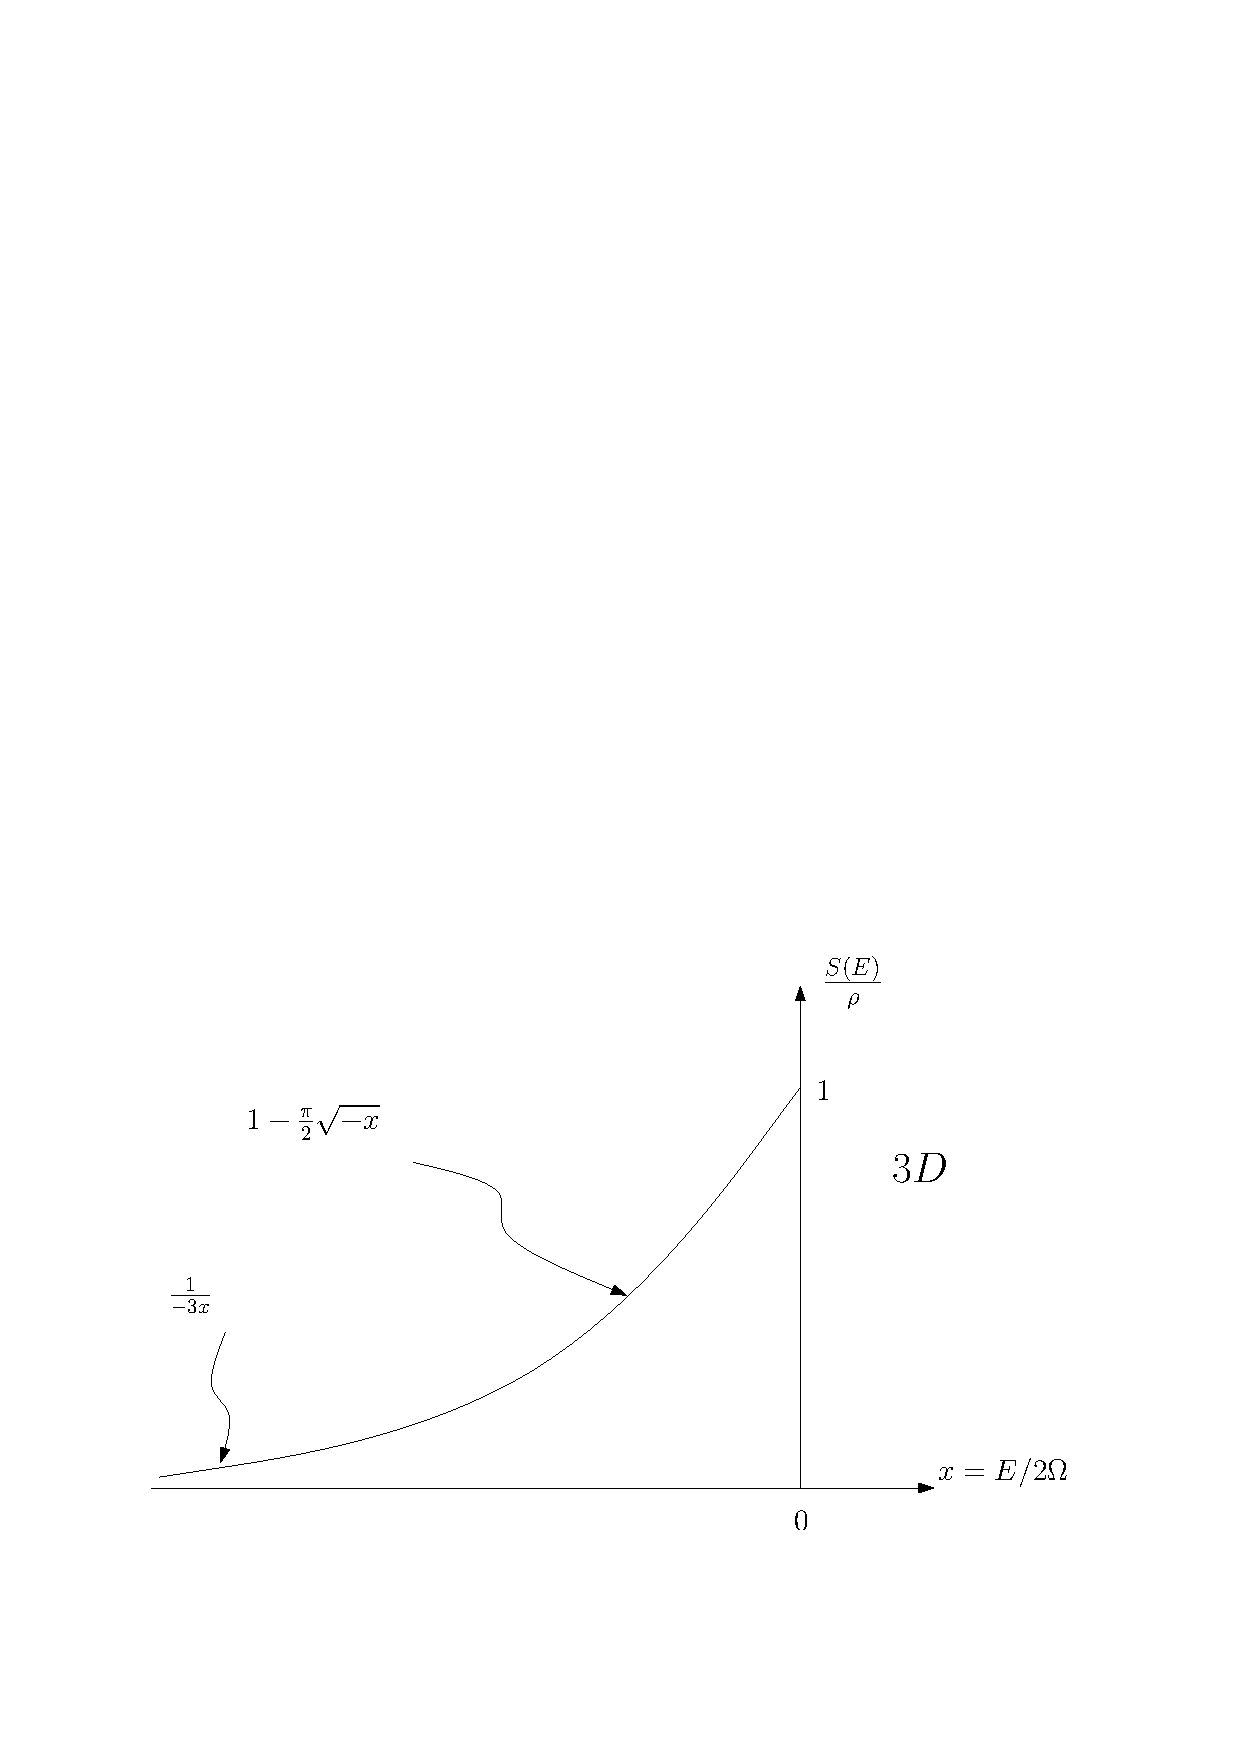
\includegraphics[width=.4\textwidth]{s3d}}\qquad
		\subfloat{\label{fig:S2d}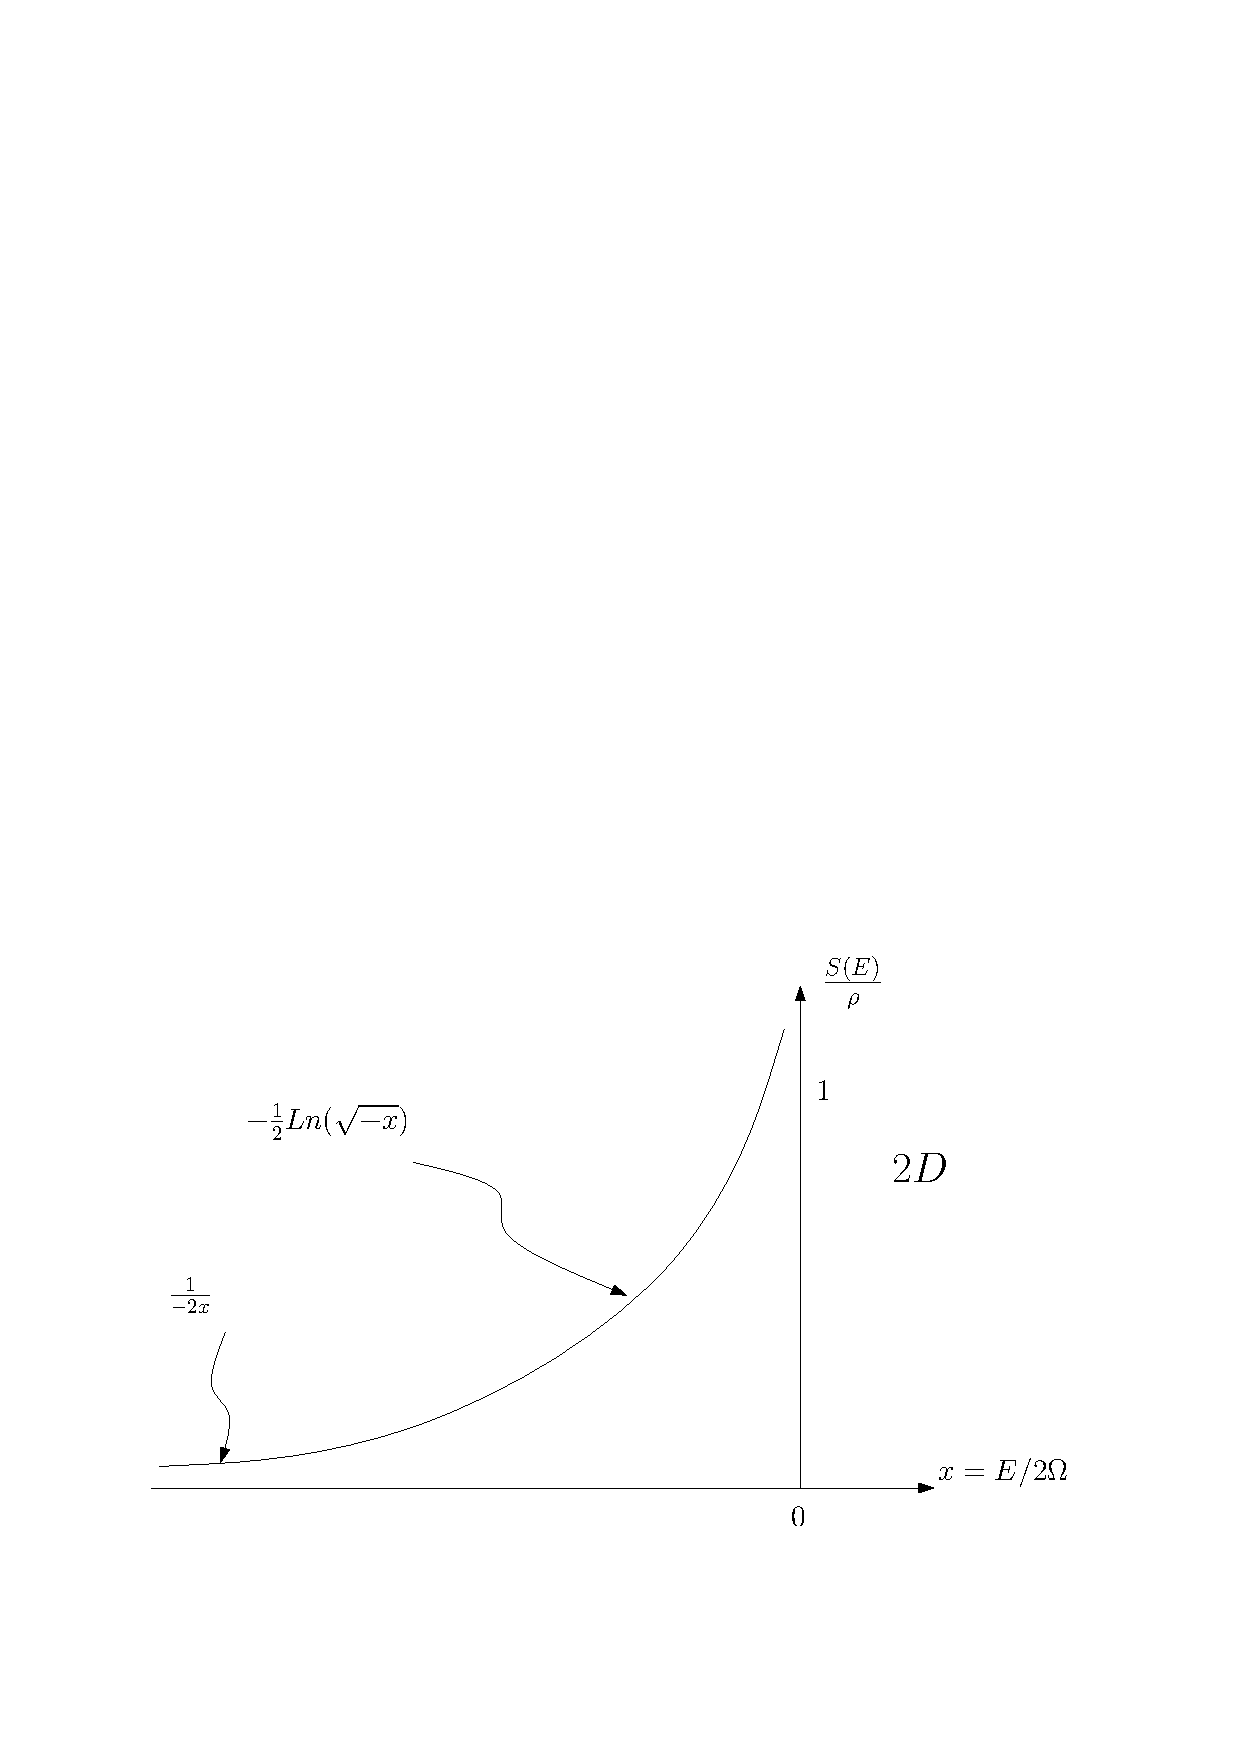
\includegraphics[width=.40\textwidth]{s2d}}
		\caption{$S(E)$ function in $3D$ and $2D$\label{fig:narrowFR}}
\end{figure}
In a $2D$ system with no frozen core, we do have since the density of states in the independent of the energy
\begin{equation}
S(E<0)=\int_{0}^{\Omega}\rho\frac{d\epsilon}{2\epsilon-E}=\frac{\rho}{2}\text{Ln}\frac{2\Omega-E}{-E}
\end{equation}
which is again valid in negative $E$ only, due to the replacement of the discrete sum over $\vk$ by an integral and the possible divergences at $\epsilon_{\vk}=E$ for positive $E$. 

The $S(E)$ curves for $3D$ and $2D$ systems are rather similar except that $S(E)$ diverges as $-1/2\text{Ln}(-E/2\Omega)$ when $E$ approaches $0_{-}$ in $2D$ while it stays finite in $3D$.  As a direct consequence, a bound state always exists for a single pair in $2D$, no matter how weak the attractive potential is, while a potential larger than a threshold is necessary in $3D$.

\subsection{Analysis of the one-pair energy}
The one-pair energy follows from 
\begin{equation}\label{eq:ssEq}
[1-v_{1}S(E_1-\epsilon_{1})][1-v_{-1}S(E_1-\epsilon_{-1})]
=\tau^2S(E_1-\epsilon_{1})S(E_1-\epsilon_{-1})
\end{equation}
in which we have set $\epsilon_{-1}=\eta_{-1}^{(\alpha)}+\eta_{-1}^{(\beta)}$ for pairs made of $(B^{\dg}_{\mathbf{k}^{},1,1},B^{\dg}_{\mathbf{k}^{},-1,-1})$ and $\epsilon_{-1}=\eta_{1}^{(\alpha)}+\eta_{-1}^{(\beta)}$ for pairs made of $(B^{\dg}_{\mathbf{k}^{},1,1},B^{\dg}_{\mathbf{k}^{},1,-1})$.

\subsubsection{In the absence of transfer $\tau=0$}
The two types of pairs are then {isolated}. Pairs in the subband $(\nu_{\alpha}=1,\nu_{\beta}=1)$ have a bound state founded that $1-v_{1}S(E_1-\eta_{1})=0$ has a solution for $E<\epsilon_{1}$.  This always happen in $2D$, no matter how weak $v_{1}$ is since $S(E)$ diverges when $E$ approach $0$. By contrast, $v_{1}$ must be larger than a threshold for a bound state to exact in $3D$.  This threshold potential is given by 
\begin{equation}
0=1-v_{\text{th}}S(0)=1-v_{\text{th}}\rho
\end{equation}
Another threshold potential is of physical interest. It corresponds to the bound state for the subbands $(1,1)$ crossing the energy of a free pair with energy $\epsilon_{-1}$ in the subbands $(-1,-1)$ or $(1,-1)$.  This potential threshold $v^{*}$ corresponds to
\begin{equation}
0=1-v^{*}S(\epsilon_{-1}-\epsilon_{1})
\end{equation}

So we end in $3D$ with
\begin{itemize}
\item no bound state below $\epsilon_{1}$ for $0<v_{1}<v_{\text{th}}$;
\item a bound state below $\epsilon_{1}$ for $E$, such that $1-v^{*}S(\epsilon_{-1}-\epsilon_{1})=0$, this bound state being above $\epsilon_{-1}$ for $v_{\text{th}}<v<v^{{*}}$ and below $\epsilon_{-1}$ for $v^{*}<v_{1}$ (see Fig \ref{fig:sDetail})
\end{itemize}
\begin{figure}[htb]
	\centering
	       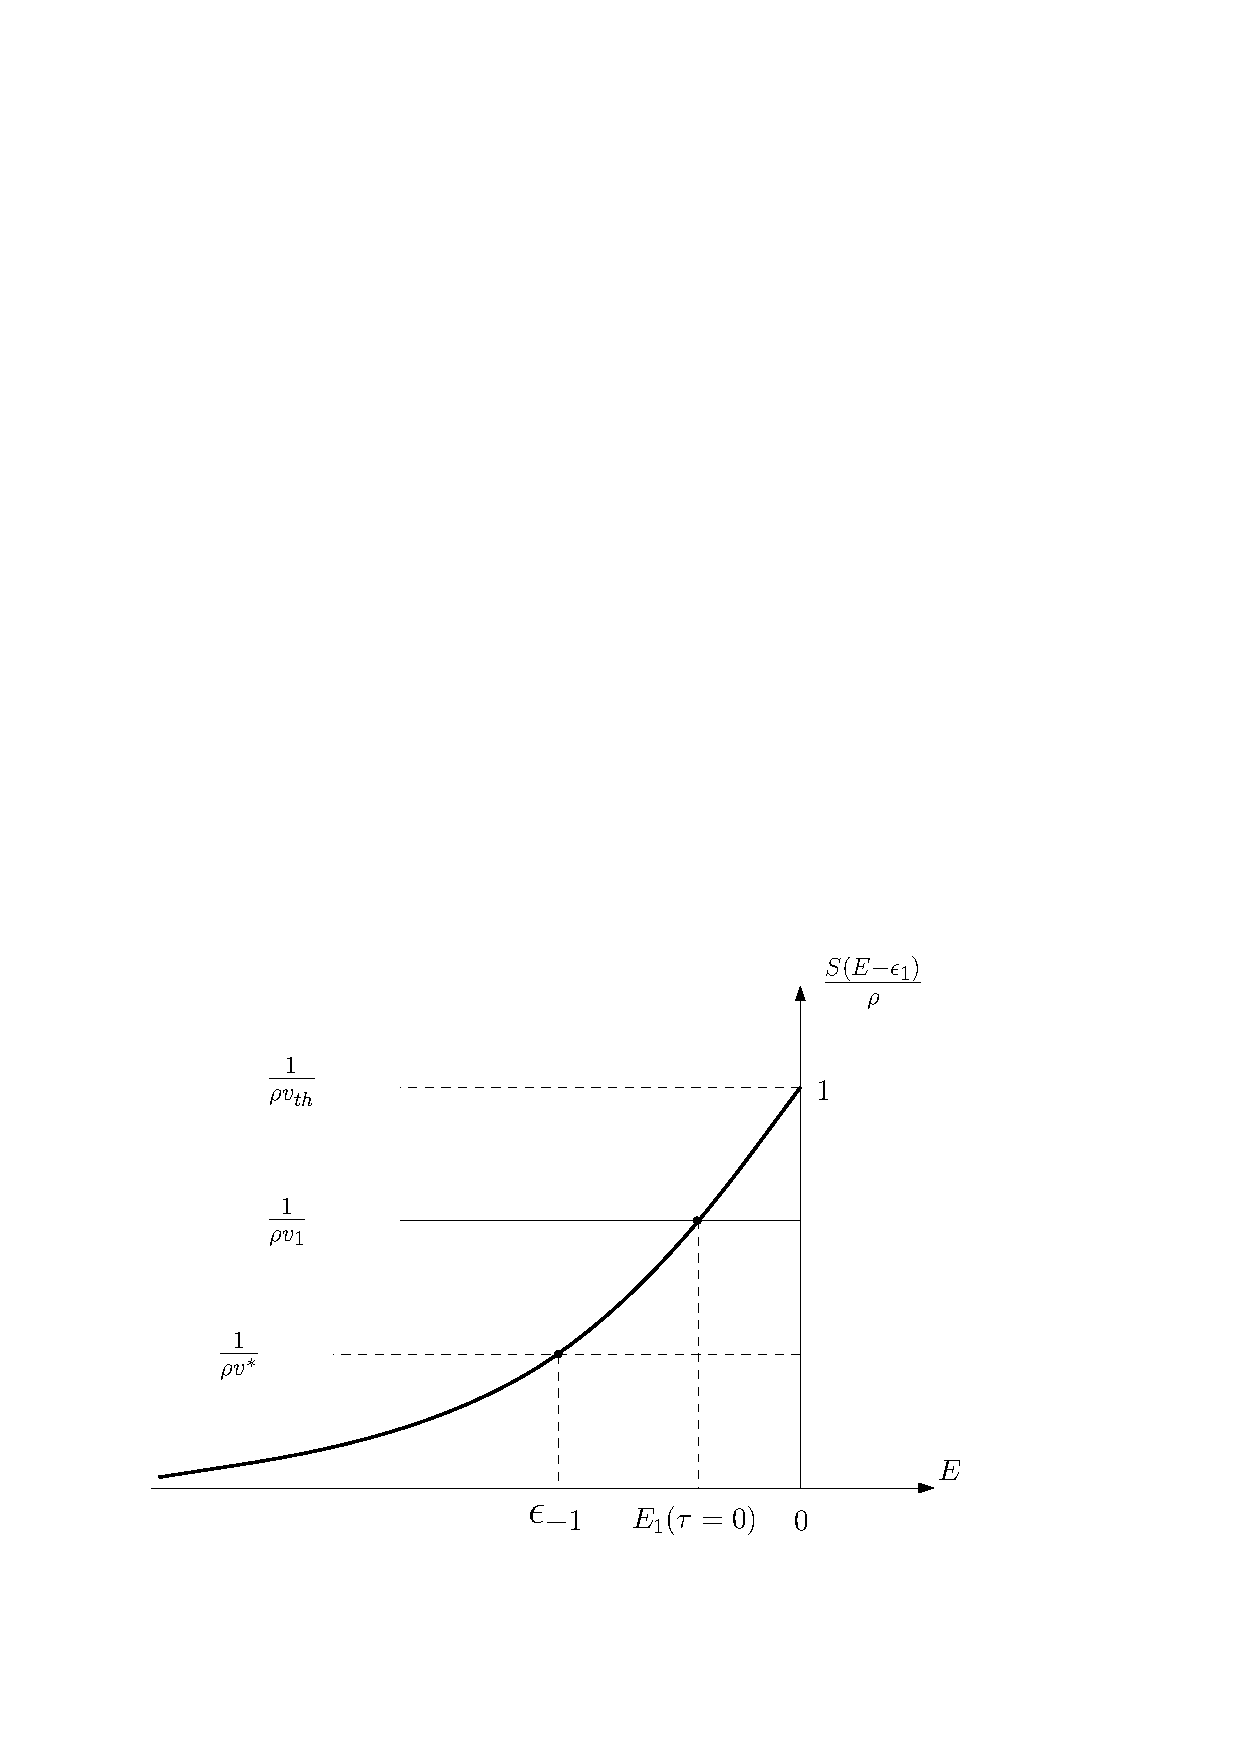
\includegraphics[width=.6\textwidth]{sDetail}
			\caption{Diagonal and non-diagonal subband interaction with shared species \label{fig:sDetail}}
\end{figure}
\subsubsection{With transfer $\tau$ but in the absence of potential within $(-1)$ subband, $v_{-1}=0$}
Eq.  \ref{eq:ssEq} for the one-pair energy follows from 
\begin{equation}
1-v_{1}S(E_1-\epsilon_{1})
=\tau^2S(E_1-\epsilon_{1})S(E_1-\epsilon_{-1})
\end{equation}
which also reads
\begin{equation}
S(E_1-\epsilon_{1})=\frac{1}{v_{1}+\tau^{2}S(E-\epsilon_{-1})}
\end{equation}
${v_{1}+\tau^{2}S(E-\epsilon_{-1})}$ can be seen as the potential of the subband $1$ dressed by its coupling to subband $-1$.  Since $S(E-\epsilon_{-1})$ varies from $\rho$ to zero when $E$ decreases from $\epsilon_{-1}$, ${1}/{\rho{}[v_{1}+\tau^{2}S(E-\epsilon_{-1})]}$ varies from $1/\rho{}v_{1}$ to $1/(\rho{}v_{1}+\rho^{2}\tau^{2})$ (see Fig \ref{fig:1rhov}). It has to be compared to $S(E-\epsilon_{1})/\rho$ shown in Fig. \ref{fig:sDetail}.  these regimes can be distinguished.  
\begin{figure}[htb]
	\centering
	       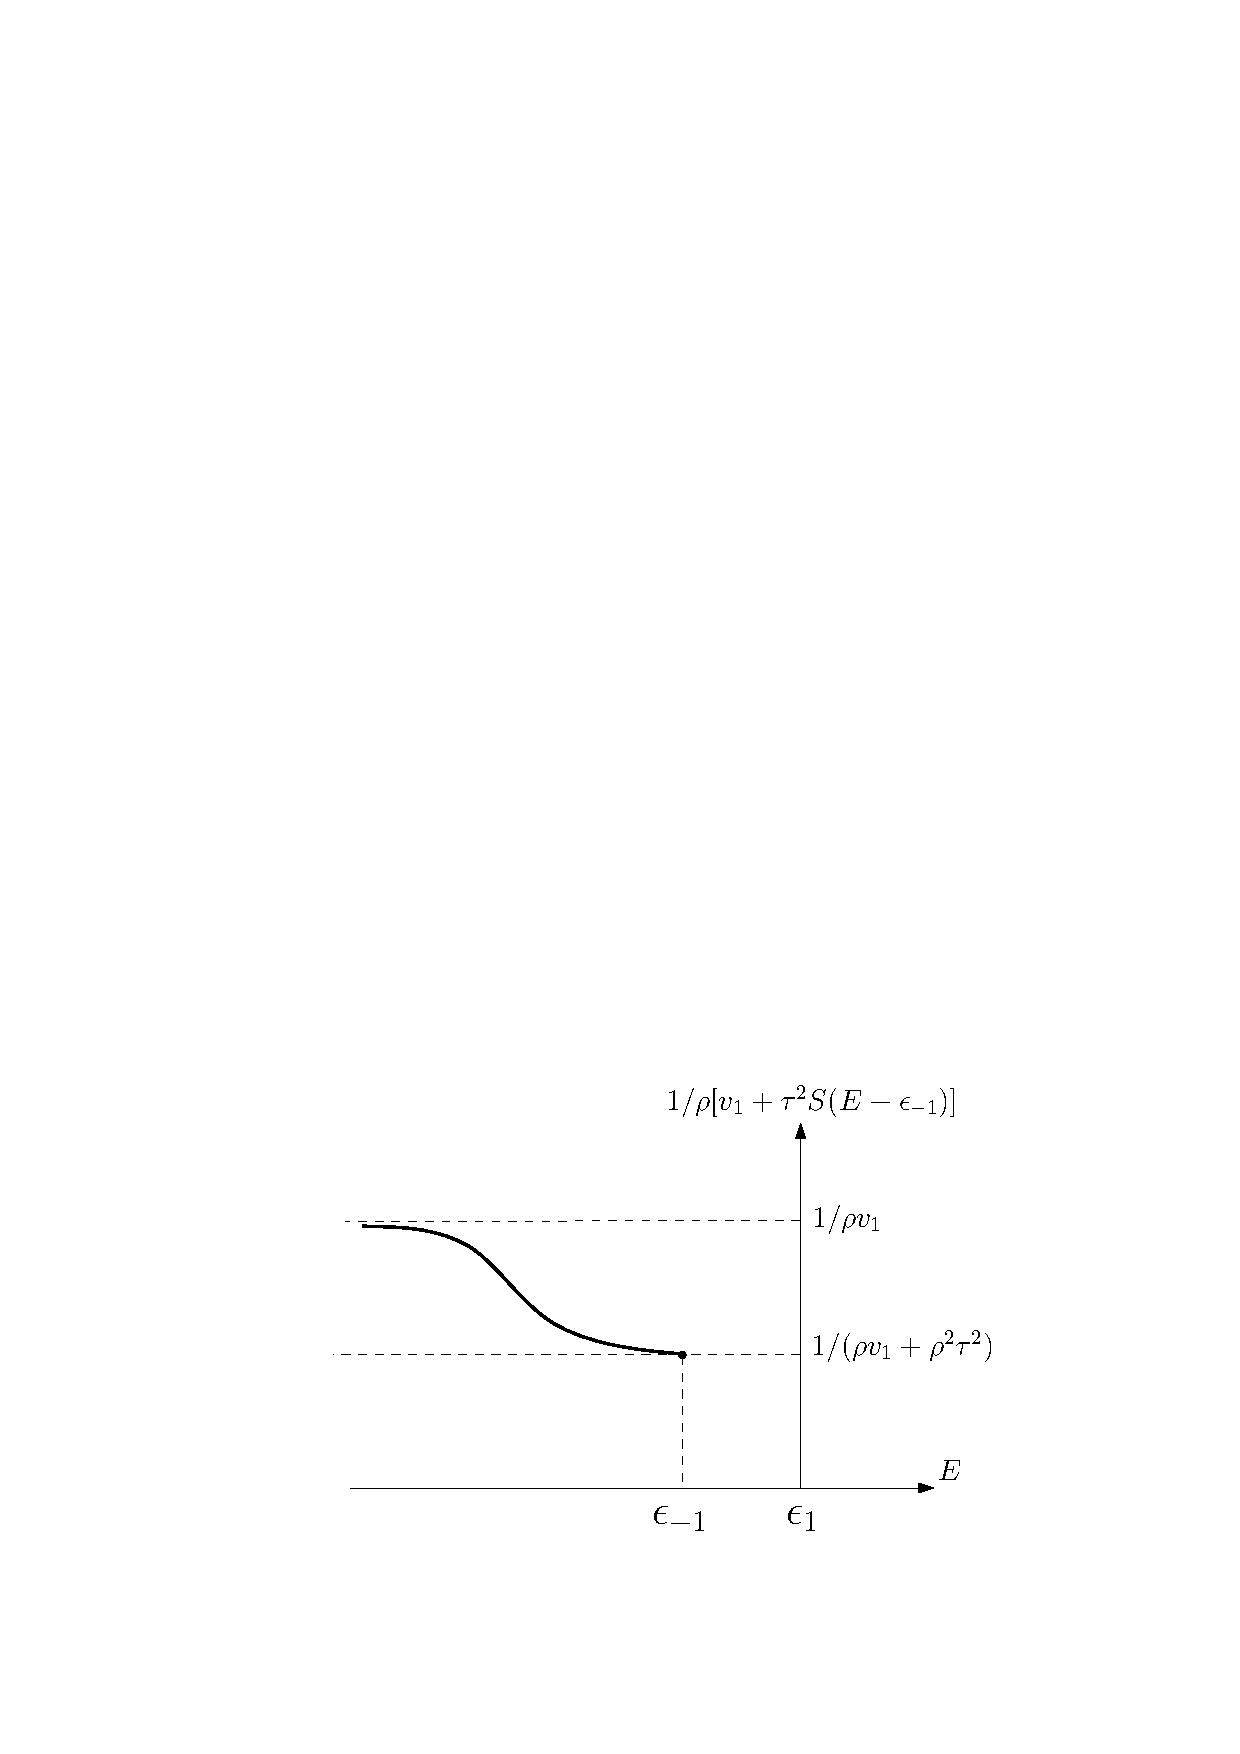
\includegraphics[width=.6\textwidth]{1rhov}
			\caption{ \label{fig:1rhov}}
\end{figure}

For $v_{\text{th}}<v_1<v_1+\tau^2\rho<v^{*}$

There is a bound state between $\epsilon_{-1}$ and $\epsilon_1$ in the uncoupled subbands and no bound state below $\epsilon_{-1}$ when the two subbands are coupled.  (See Fig. \ref{fig:noBound})

\begin{figure}[htb]
	\centering
	       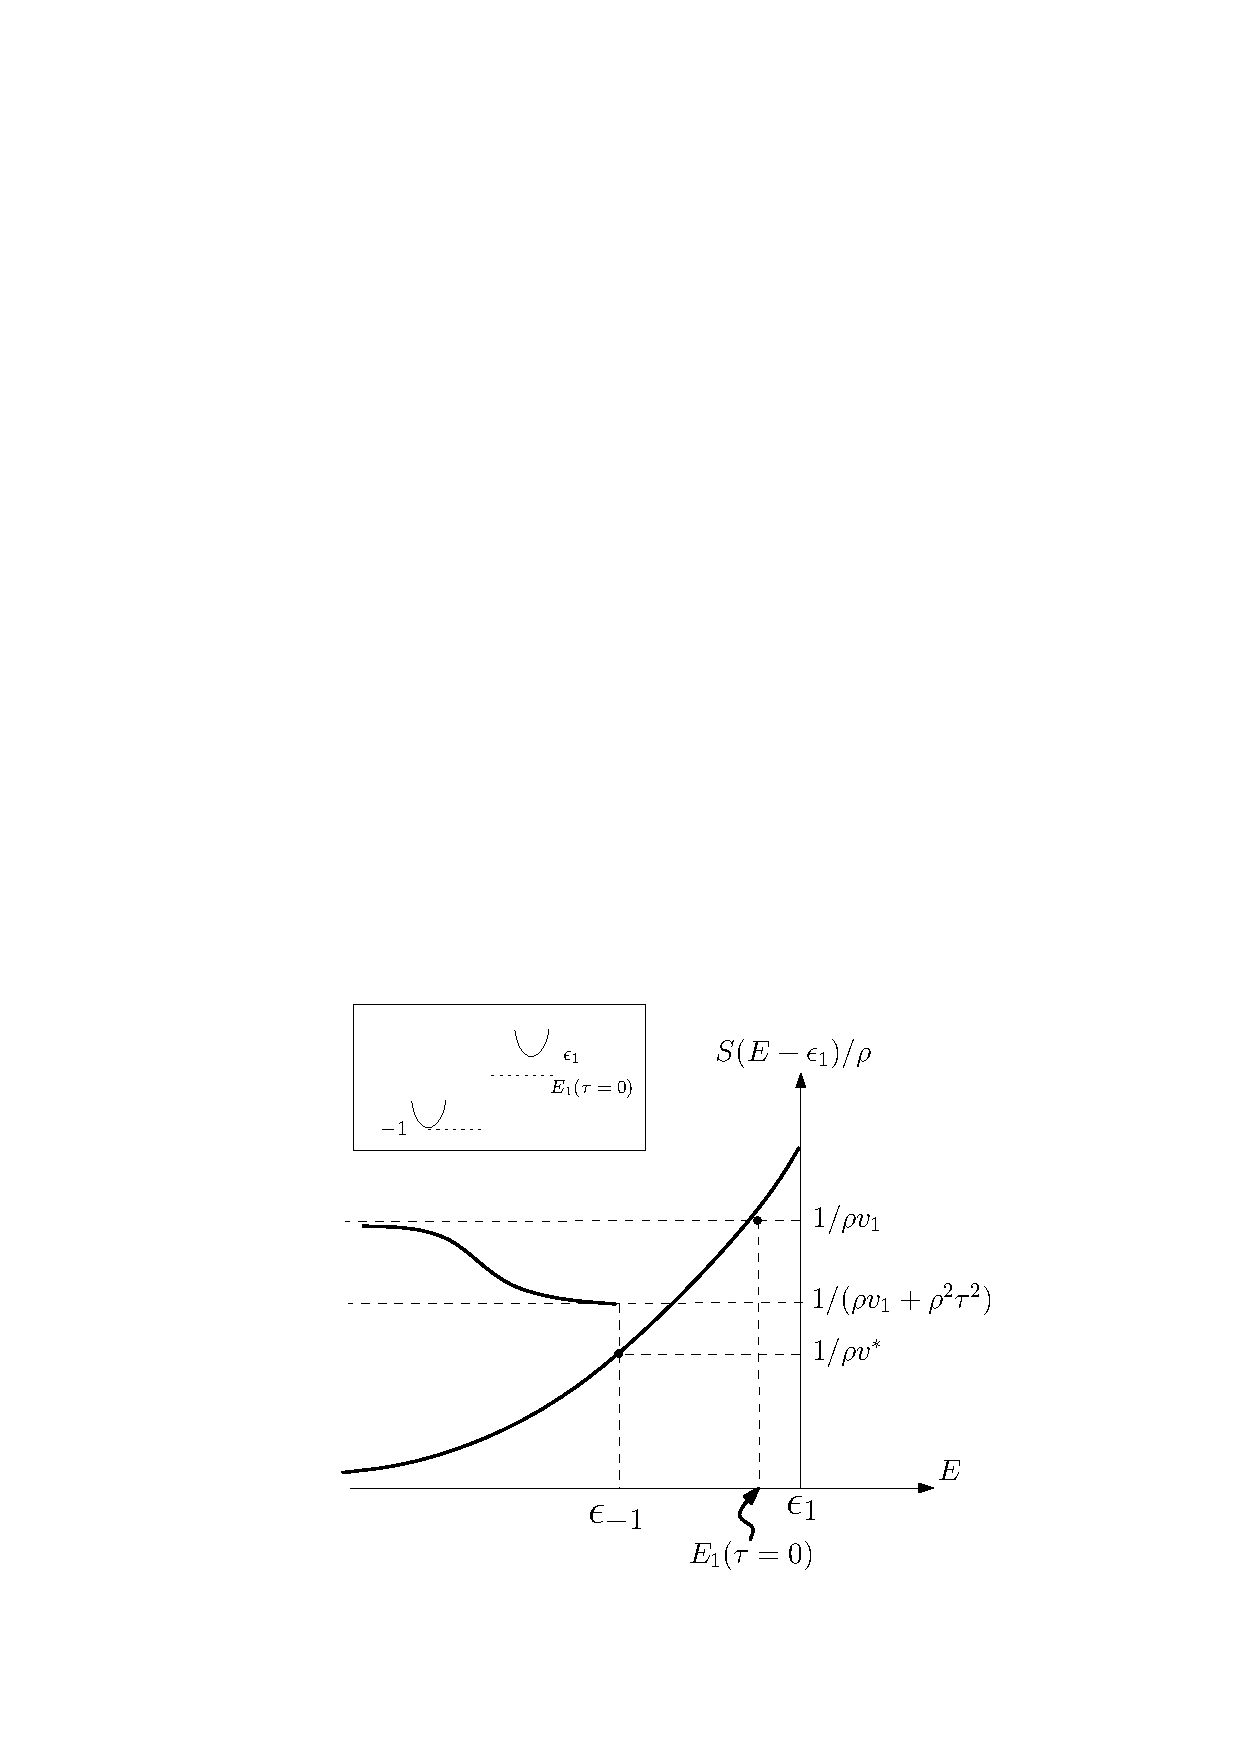
\includegraphics[width=.6\textwidth]{noBound}
			\caption{\label{fig:noBound}}
\end{figure}

For $v_{\text{th}}<v_1<v^{*}<v_1+\tau^2\rho$

There is a bound state between $\epsilon_{-1}$ and $\epsilon_1$ for the uncoupled subbands and a bound state below $\epsilon_{-1}$ for the two coupled subbands.  (See Fig. \ref{fig:bound})

\begin{figure}[htb]
	\centering
	       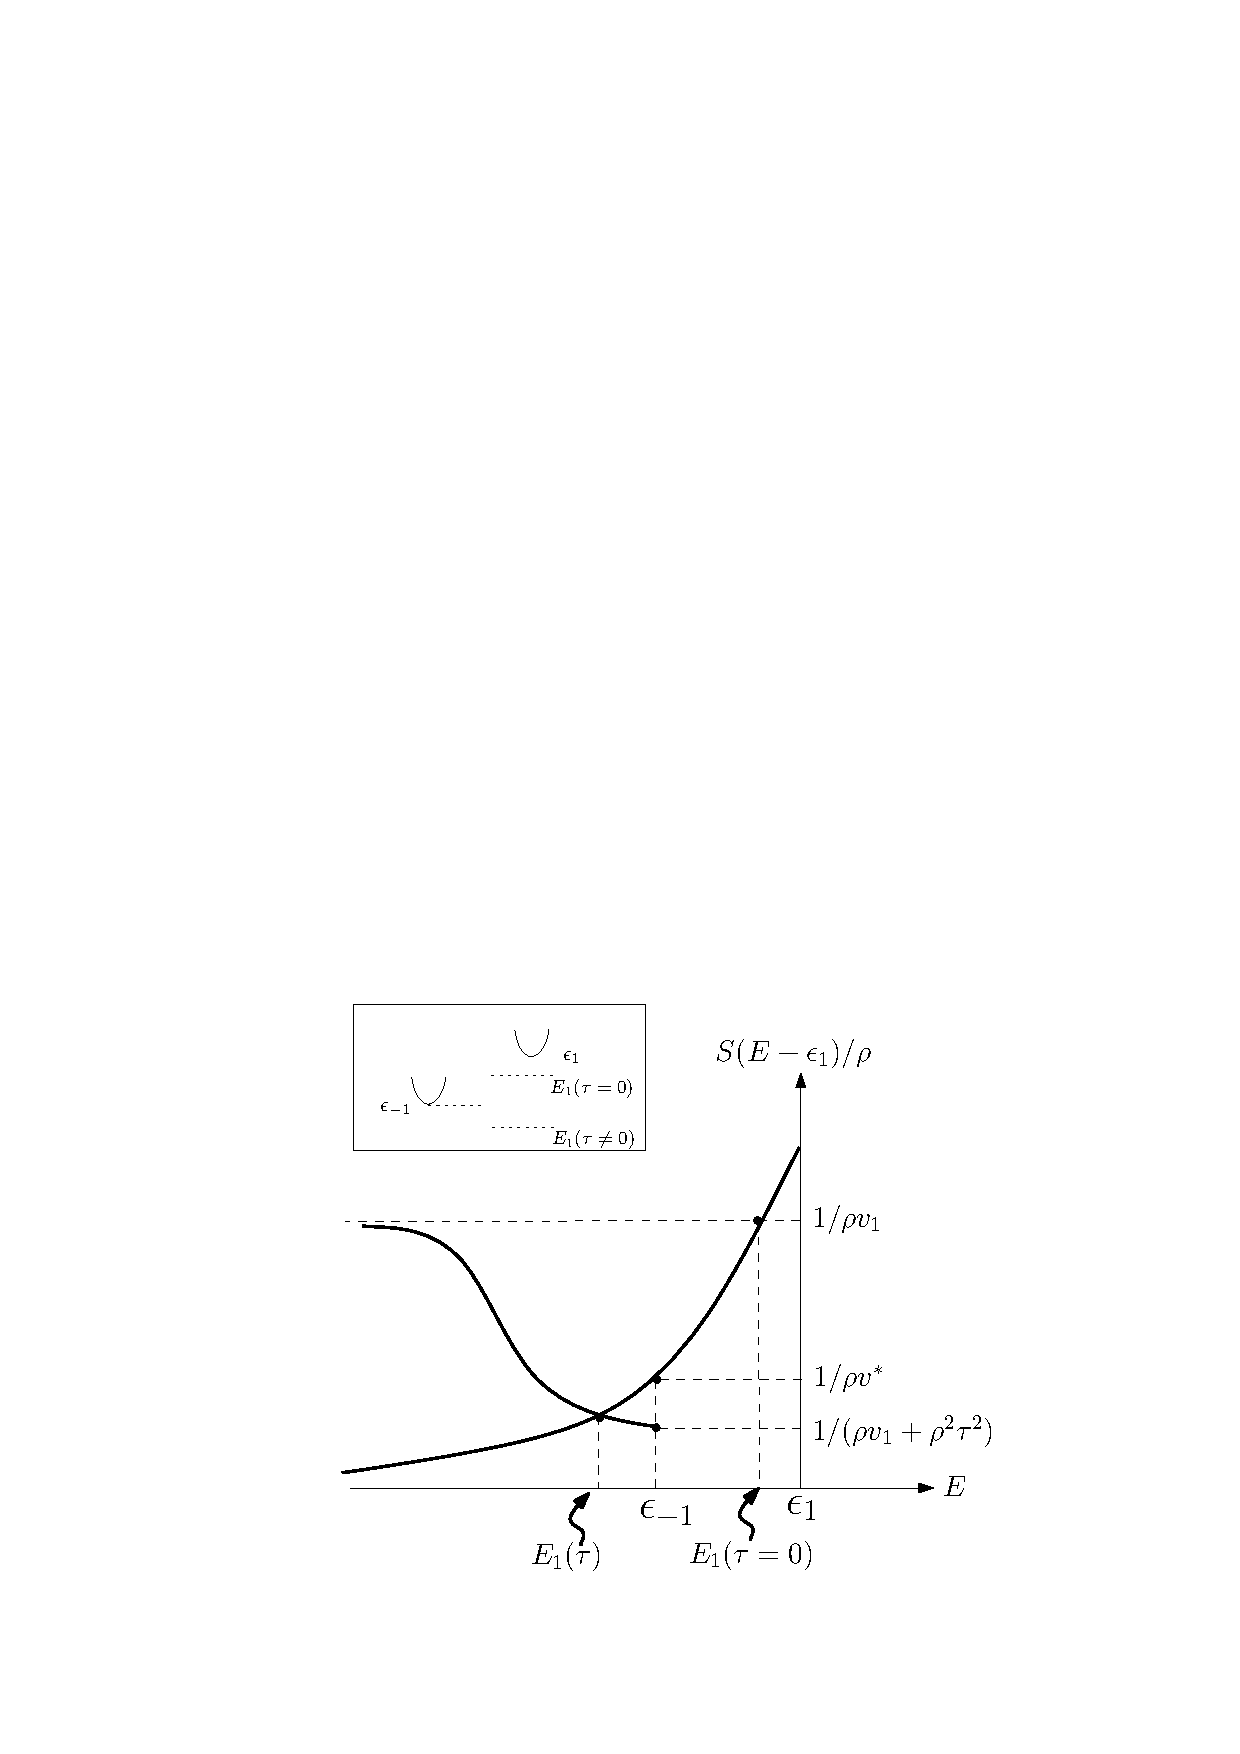
\includegraphics[width=.6\textwidth]{bound}
			\caption{\label{fig:bound}}
\end{figure}

For $v_{\text{th}}<v^{*}<v_1<v_1+\tau^2\rho$

There is a bound state below $\epsilon_{-1}$ for the uncoupled subbands as well as for the  coupled subbands.  (See Fig. \ref{fig:bound2})

\begin{figure}[htb]
	\centering
	       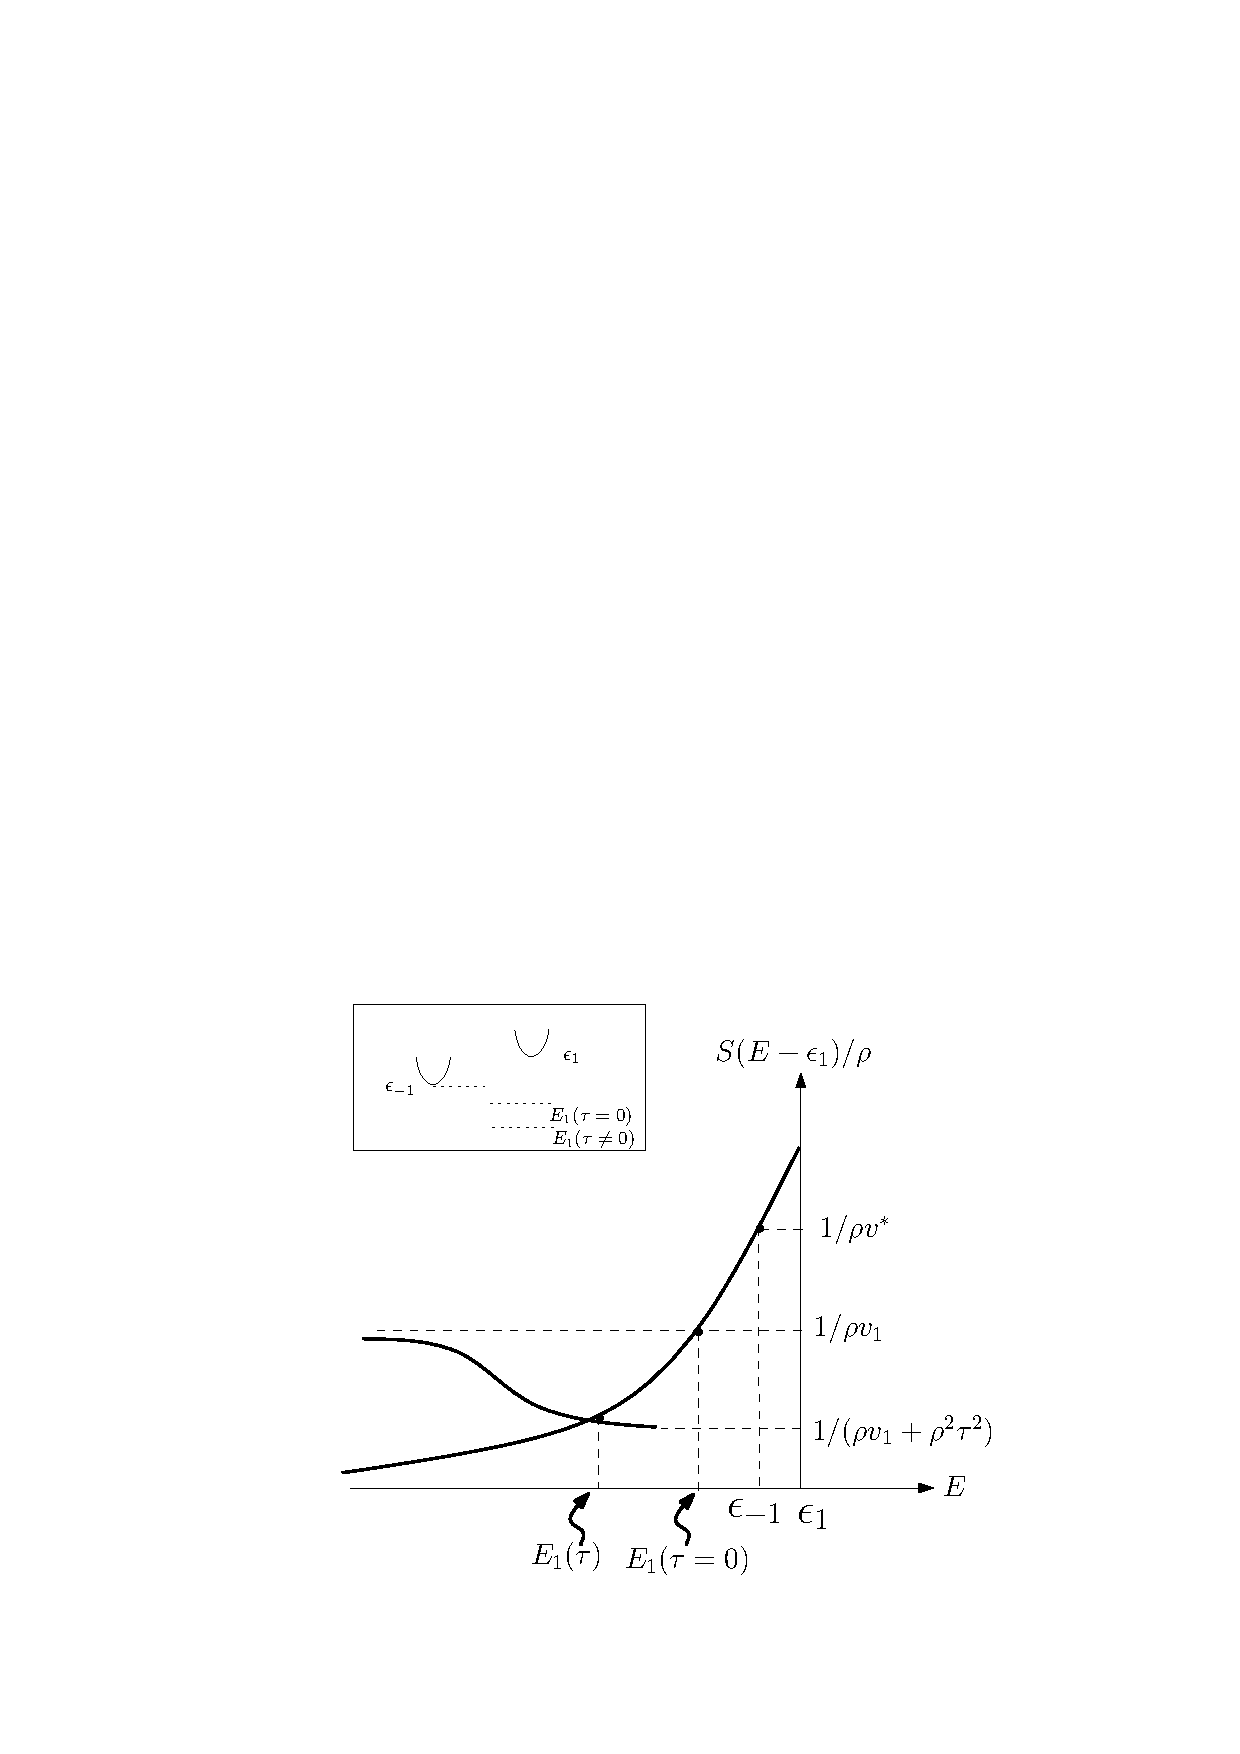
\includegraphics[width=.6\textwidth]{bound2}
			\caption{\label{fig:bound2}}
\end{figure}

As expected, a finite transfer between subbands $1$ and $-1$ helps to form a bound state below $\epsilon_{-1}$ for a given coupling $v_{1}$ in subband $1$. By increasing the magnetic field by the fermionic atoms $\alpha$ and $\beta$, we can actually decrease the energy difference $\epsilon_{1}-\epsilon_{-1}$. So we get the following sequences show in Fig. \ref{fig:seqS} when the magnetic field increases for two coupled subbands in the absences of the potential between the atoms of subbands $(-1)$.
\begin{figure}[htb]
	\centering
	       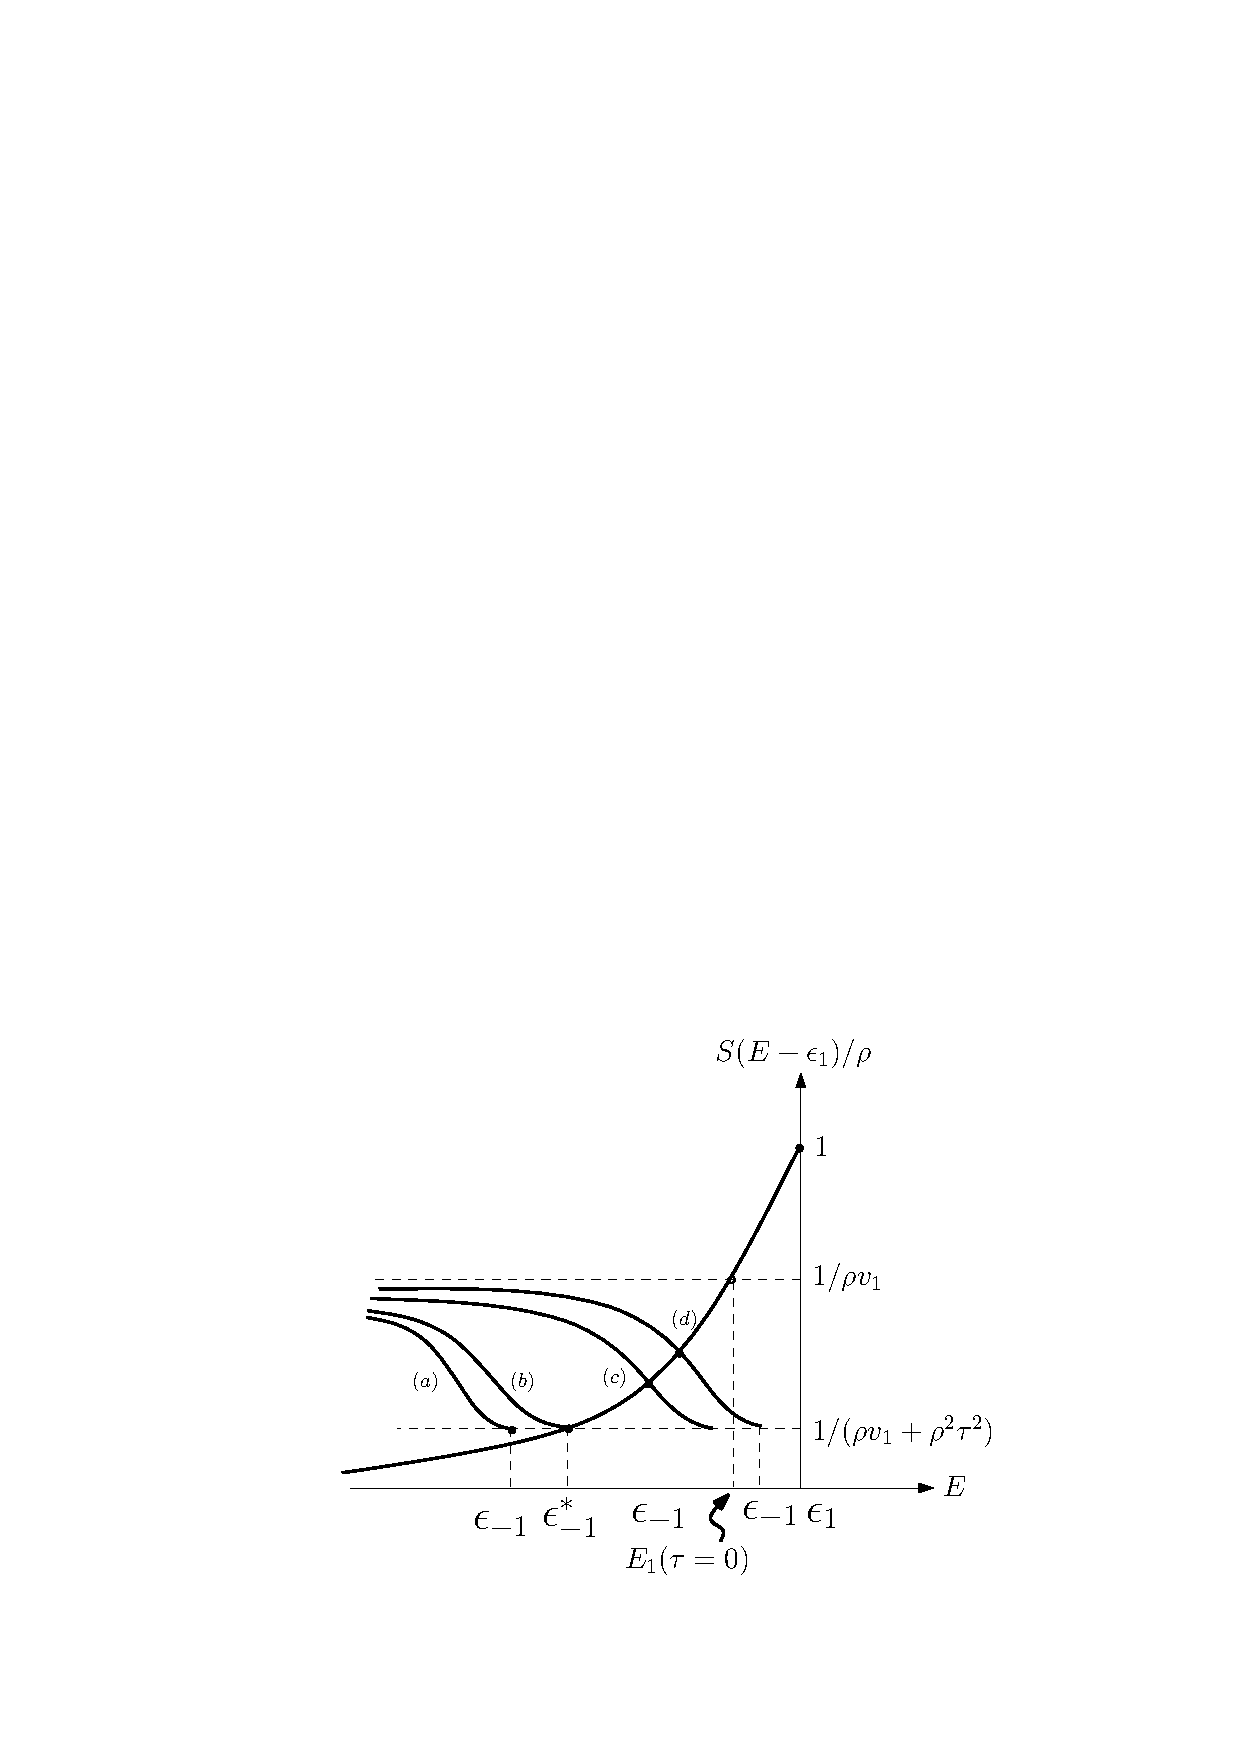
\includegraphics[width=.6\textwidth]{seqS}
			\caption{\label{fig:seqS}}
\end{figure}

\begin{description}
 \item[(a)] The energy of subband $(-1)$ is too low to possibly have a bound state induced by the attractive potential in subband $(-1)$, even in the presence of subband coupling.
 \item[(b)] It corresponds  to the threshold for appearance of a bound state below $\epsilon_{{-1}}$.  It corresponds to $\epsilon_{-1}$ reaching $\epsilon_{-1}^{*}$ given by 
 \begin{equation}
 S(\epsilon^{*}_{-1}-\epsilon_{1})=\frac{1}{v_{1}+\tau^{2}\rho}
 \end{equation}
 \item[(c)] A bound state below $\epsilon_{-1}$ exists in the presence of inter-band coupling but not without it.
 \item[(d)] The energy difference $\epsilon_{-1}-\epsilon_{1}$ is small enough to have the bound state $E_{1}(\tau=0)$ of the subband $(1)$ alone, below $\epsilon_{-1}$

\end{description}

\subsubsection{With transfer $\tau$ and coupling in the two subbands}
In order to better see the effect of the transfer coupling $\tau$ and the $v_{-1}$ digonal coupling, it is convenient to rewrite Eq. \ref{eq:ssEq} for the one-pair energy as 
\begin{equation}\label{eq:ssEq2}
S(E-\epsilon_1)=\frac{1}{\displaystyle v_1+\frac{\tau^2S(E-\epsilon_{-1})}{1-v_{-1}S(E-\epsilon_{-1})}}
\end{equation}
The physically relevant problem is to look for a bound state below $\epsilon_{-1}$ when the coupling $v_{-1}$ in the $(-1)$ subband is not strong enough to provide one, i.e., $1<1/\rho{}v_{-1}$. 

When $E$ increases from $-\infty$ to $\epsilon_{-1}$, $S(E-\epsilon_{-1})$ increases from $0$ to $1/\rho$.  So the R.H.S. in Eq. \ref{eq:ssEq2} decreases from $1/v_1$ to $1/[v_1+\tau^2\rho/(1-v_{-1}\rho)]$, which is larger than $1/(v_1+\tau^2\rho)$ since $v_{-1}\rho$ is positive.  As a result, we essentially have the same three behaviors as the one for $v_{-1}=0$, with just $1/(\rho{}v_1+\tau^2\rho^2)$ replaced by $1/[\rho{}v_1+\tau^2\rho^2/(1-v_{-1}\rho)]$.  We see that the effect of introducing a weak $v_{-1}$ coupling in subband $-1$ is essentially to enhance the transfer coupling $\tau$. 

\subsubsection{Complete picture}
The above discussion shows that we need a potential $v$ in the subband $1$ large enough to have a bound state in this subband alone, i.e., a bound state with energy lower than $\epsilon_1$.  The threshold condition for this to happen then reads
\begin{equation}
\frac{1}{v_1}<\rho<S(0)
\end{equation}
with $S(E)$ defined in Eq. \ref{eq:Sdef}.  

We of course need a large potential if we want this bound state to be below the energy of a free pair in the subband $-1$, i.e., a bound state with energy lower than $\epsilon_{-1}$.  The threshold condition then reads
\begin{equation}
\frac{1}{v_1}<S(\epsilon_{-1}-\epsilon_1)=S(0)
\end{equation}
If we now take into account possible transfer between subbands $1$ and $2$ and the fact that the subbands $(-1)$ also have an attractive potential, although too weak to produce a bound state in these subbands alone. The above condition transforms into 
\begin{equation}
\frac{1}{\tilde{v}_1}<S(\epsilon_{-1}-\epsilon_1)
\end{equation}
when the effective coupling $\tilde{v}_1$ of subband $(1)$ induced by the $\tau$ transfer and the $v_{-1}$ coupling reads as 
\begin{equation}
\tilde{v}_1=v_1+\frac{\tau^2\rho}{v_{1}+\tau^{2}\rho}
\end{equation}
This effective coupling is visualized for small $v_{-1}$ by the set of ladder diagrams of Fig. \ref{fig:ladder}


\begin{figure}[htb]
	\centering
	       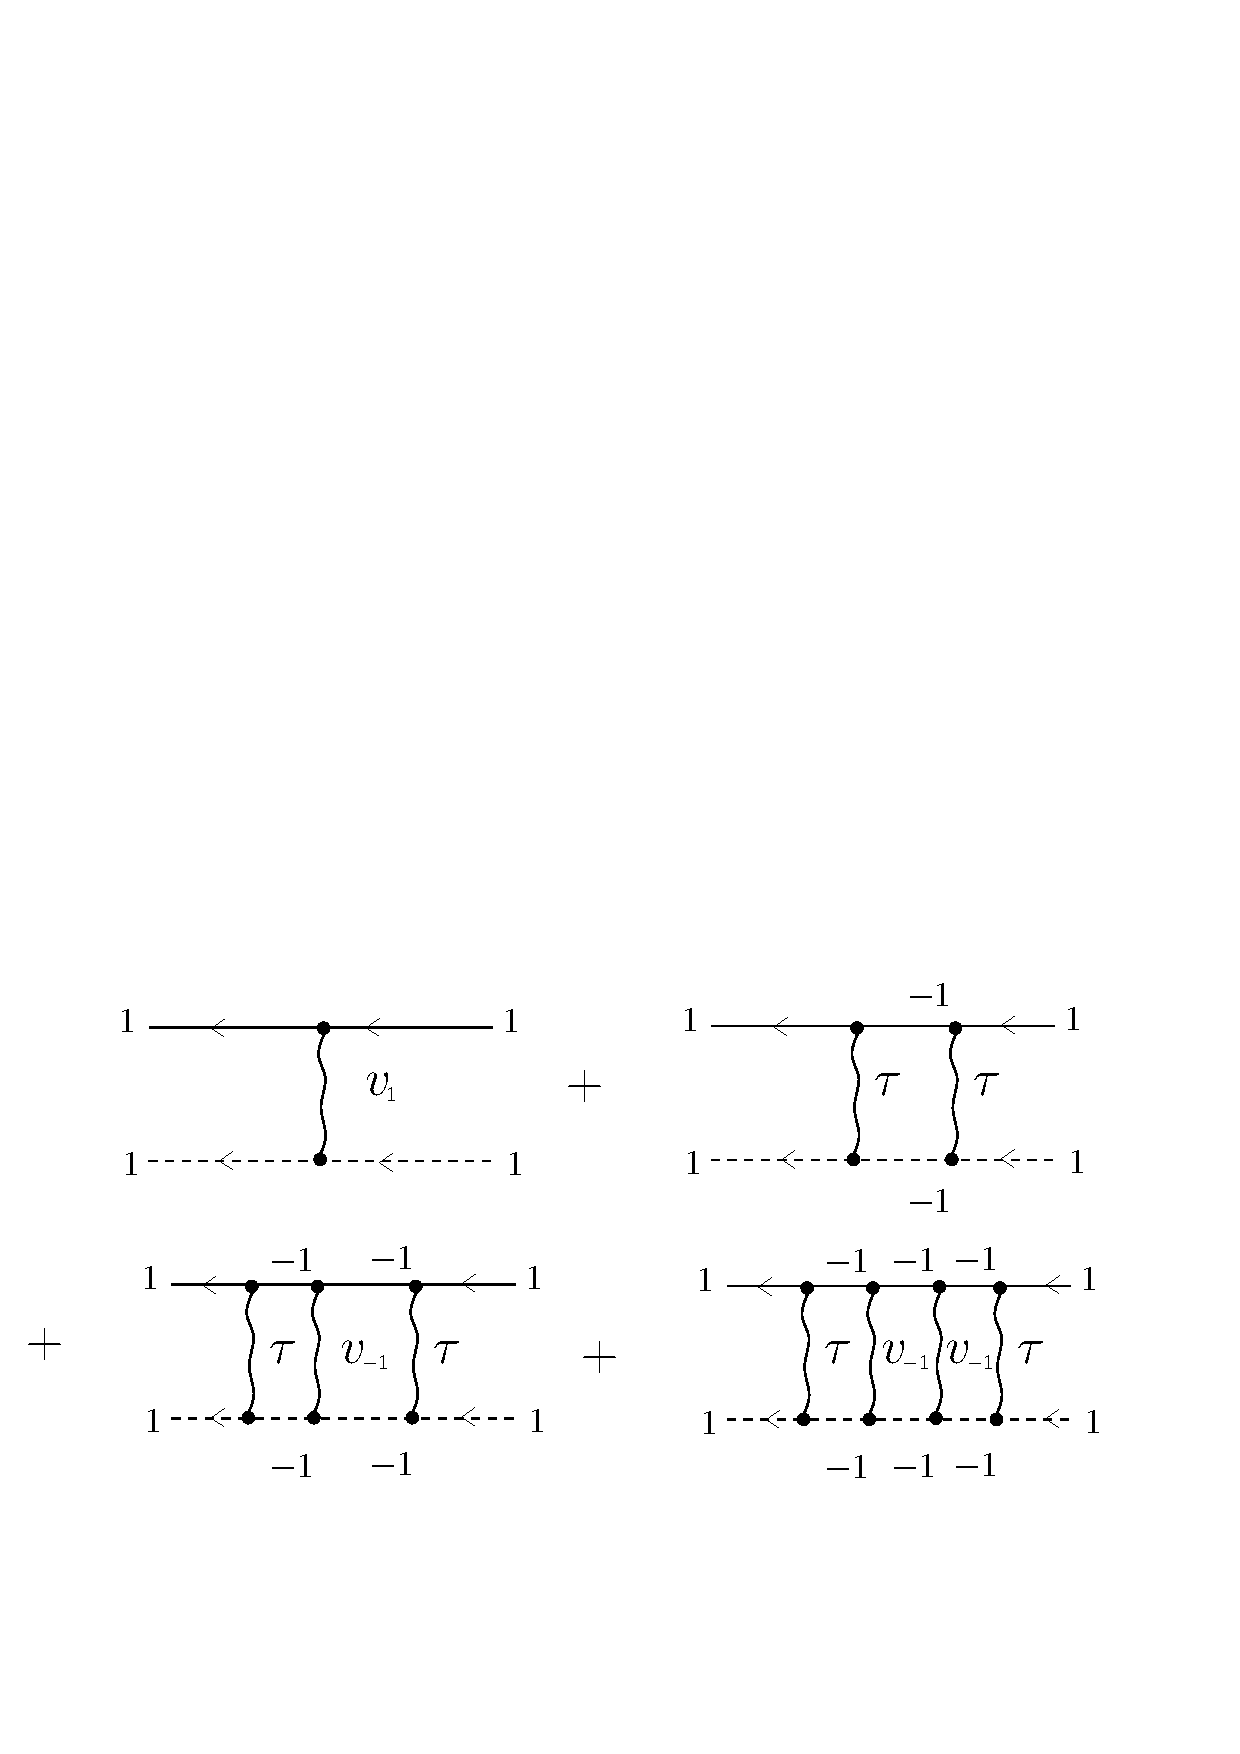
\includegraphics[width=.6\textwidth]{ladder}
			\caption{\label{fig:ladder}}
\end{figure}

We see, as comewhat expected, that an interband transfer helps to have a bound state below $\epsilon_{-1}$, this effect being enhanced by the existence of a weak coupling in subband $(-1)$.  

We are now going consider two fermion pairs and study how their energy $E_2$ varies compared to every $2E_1$ of two single pairs, when the tranfer $\tau$ and the coupling $v_{-1}$ in subband $-1$ are introduced into the problem.  We will 
pay particular attention to the effect of Pauli blocking when the pairs show a common fermion, i.e., when they are made of $B^{\dg}_{\mathbf{k}^{ },1,1}$ and $B^{\dg}_{\mathbf{k}^{ },1,-1}$, compared to the case when their fermions are totally different, i.e., when they are made of $B^{\dg}_{\mathbf{k}^{ },1,1}$ and $B^{\dg}_{\mathbf{k}^{ },-1,-1}$.

\section{Two-pair ground state}
We now consider two pairs of fermions $\alpha$ and $\beta$, these fermions possibly being in subbands $\nu=1$ or $\nu=-1$.  As in the case of a single pair, we will first study the case when these pairs are made with different fermions.  So, the Pauli exclusion principle holds among pairs $B^{\dg}_{\mathbf{k}_1^{ },\nu,\nu}$ and $B^{\dg}_{\mathbf{k}_2^{ },-\nu,-\nu}$.

\subsection{Pairs made of $B^{\dg}_{\mathbf{k}^{ },1,1}$ and $B^{\dg}_{\mathbf{k}^{ },-1,-1}$}
The relevant potential here are $V$ and $T$ given in Eqs. (\ref{eq:V}, \ref{eq:T}). The commutation of Eq.  \ref{eq:h0B} gives the free part as 
\begin{equation}\label{eq:H0B}
H_0\,B^{\dg}_{\mathbf{k}_{1},\nu_1,\nu_1}B^{\dg}_{\mathbf{k}_{2},\nu_2,\nu_2}|0\rangle=
(2\epsilon_{\vk_1}+\epsilon_{\nu_1}+2\epsilon_{\vk_2}+\epsilon_{\nu_2})B^{\dg}_{\mathbf{k}_{1},\nu_1,\nu_1}B^{\dg}_{\mathbf{k}_{2},\nu_2,\nu_2}|0\rangle
\end{equation}
with again $\epsilon_{\nu}=\eta_{\nu}^{(\alpha)}+\eta_{\nu}^{(\beta)}$. To get the potentials on these two-pair states, we use Eqs. (\ref{eq:bb}-\ref{eq:db}).  These give
\begin{equation}\label{eq:VT1}
(V+T)B^{\dg}_{\mathbf{k}_{1},\nu,\nu}B^{\dg}_{\mathbf{k}_{2},\nu,\nu}|0\rangle=(1-\delta_{\vk_1\vk_2})I^{\dg}_{\nu}\Big(w_{\vk_2}B^{\dg}_{\mathbf{k}_{1},\nu,\nu}+w_{\vk_1}B^{\dg}_{\mathbf{k}_{2},\nu,\nu}\Big)|0\rangle
\end{equation}
where we have set
\begin{equation}
I^{\dg}_{\nu}=v_{\nu}\beta^{\dg}_{\nu\nu}+\tau{}\beta^{\dg}_{-\nu-\nu}
\end{equation}
with $\beta^{\dg}_{\nu\nu}$ defined in Eq. \ref{eq:beta}. Note that the $(1-\delta_{\vk_1,\vk_2})$ factor comes from Pauli blocking.  It is necessary to ensure that the R.H.S. cancels, as the L.H.S. does, when $\vk_1=\vk_2$.  By contrast, this factor does not exist when the pairs are made with different fermions.  We then find,
\begin{equation}
(V+T)B^{\dg}_{\mathbf{k}_{1},\nu,\nu}B^{\dg}_{\mathbf{k}_{2},-\nu,-\nu}|0\rangle
=-\Big(w_{\vk_2}B^{\dg}_{\mathbf{k}_{1},\nu,\nu}I^{\dg}_{-\nu}+w_{\vk_1}B^{\dg}_{\mathbf{k}_{2},-\nu,-\nu}I^{\dg}_{\nu}\Big)|0\rangle
\end{equation}
This equation can be symmetrized and written similar to Eq. \ref{eq:VT1} through
\begin{equation}
\begin{split}
&(V+T)\Big(B^{\dg}_{\mathbf{k}_{1},\nu,\nu}B^{\dg}_{\mathbf{k}_{2},-\nu,-\nu}+B^{\dg}_{\mathbf{k}_{1},-\nu,-\nu}B^{\dg}_{\mathbf{k}_{2},\nu,\nu}\Big)|0\rangle\\
=&-I^{\dg}_{\nu}\Big(w_{\vk_2}B^{\dg}_{\mathbf{k}_{1},-\nu,-\nu}+w_{\vk_1}B^{\dg}_{\mathbf{k}_{2},-\nu,-\nu}\Big)|0\rangle\\
&-I^{\dg}_{-\nu}\Big(w_{\vk_2}B^{\dg}_{\mathbf{k}_{1},\nu,\nu}+w_{\vk_1}B^{\dg}_{\mathbf{k}_{2},\nu,\nu}\Big)|0\rangle
\end{split}
\end{equation}
\subsubsection{In the absence of transfer coupling, $\tau=0$}
Let us first drop the transfer coupling between subbands $(+1)$ and $(-1)$ and see how the exact 2-pair solution found by Richardson \cite{Richardson1, Richardson2, Richardson3} and by Gaudin \cite{Gaudin} can be recovered from the above equations. 

By dropping the $\nu$ indices for simplicity, we look for the solution of $(H_0+V-E_2)|\Psi_2\rangle=0$ as $|\Psi_2\rangle=\sum_{\vk_1,\vk_2}w_{\vk_1}w_{\vk_2}\phi_{\vk_1,\vk_2}B^{\dg}_{\vk_1}B^{\dg}_{\vk_2}|0\rangle$.  Here $w_{\vk}$ factors come from the fact that this two-pair eigenstate is expected to be made of $\vk$ states feeling the potential.  We first note, using Eq. \ref{eq:VT1}, that
\begin{equation}
V|\Psi_2\rangle=
-v\sum_{\vk_1,\vk_2}w_{\vk_1}w_{\vk_2}\phi_{\vk_1,\vk_2}({w_{\vk_2}}B^{\dg}_{\vk_1}+{w_{\vk_1}}B^{\dg}_{\vk_2})\sum_{\vp}w_{\vp}B^{\dg}_{\vp}|0\rangle
\end{equation}
can be rewritten by exchange $(\vk_2,\vp)$ and $(\vk_1,\vp)$, as 
\begin{equation}\label{eq:VPsi2}
V|\Psi_2\rangle=-v\sum_{\vk_1,\vk_2}w_{\vk_1}w_{\vk_2}B^{\dg}_{\vk_1}B^{\dg}_{\vk_2}
\Big[\sum_{\vp}w_{\vp}(\phi_{\vk_1\vp}+\phi_{\vk_2\vp})-\phi_{\vk_1,\vk_2}-\phi_{\vk_2,\vk_1}\Big]|0\rangle
\end{equation}
in which we have dropped the $w_{\vk_1}$ factor in front of $\phi_{\vk_1,\vk_1}$ since $w_{\vk_1}^2=w_{\vk}$; and similarly in $\phi_{\vk_2,\vk_2}$.

Using Eqs. (\ref{eq:H0B}, \ref{eq:VPsi2}), the Schr\"odinger equation then appears as $0=\sum_{\vk_1,\vk_2}w_{\vk_1}w_{\vk_2}B^{\dg}_{\vk_1}B^{\dg}_{\vk_2}F_{\vk_1,\vk_2}|o\rangle$ with
\begin{equation}
F_{\vk_1,\vk_2}=(2\epsilon_{\vk_1}+2\epsilon_{\vk_2}-E_2)\phi_{\vk_1,\vk_2}
-v\Big[\sum_{\vp}w_{\vp}(\phi_{\vk_1,\vp}+\phi_{\vk_2,\vp})-\phi_{\vk_1,\vk_1}-\phi_{\vk_2,\vk_2}\Big]
\end{equation}
By projecting the Schr\"odinger equation on $\langle0|B_{\vp_2,1,1}B_{\vp_1,1,1}$ and by noting that 
\begin{equation}
\langle0|B_{\vp_2,1,1}B_{\vp_1,1,1}B^{\dg}_{\vk_1,1,1}B^{\dg}_{\vk_2,1,1}|0\rangle
=\delta_{\vp_1\vk_1}\delta_{\vp_2\vk_2}+\delta_{\vp_1\vk_2}\delta_{\vp_2\vk_1}-2\delta_{\vp_1\vk_1}\delta_{\vp_2\vk_2}\delta_{\vp_1\vp_2}
\end{equation}
We get the prefactor $F_{\vk_1\vk_2}$ for $\vp_1\neq\vp_2$ as $0=F_{\vp_1\vp_2}+F_{\vp_2\vp_1}$ while for $\vp_1=\vp_2$. This prefactor is undefined, which is unimportant since the two-pair state $B^{\dg}_{\vp_1}B^{\dg}_{\vp_2}|0\rangle$ cancels anyway.  

This leads us to seek for a solution symmetrical in $(\vp_1,\vp_2)$, this solution then fulfilling 
\begin{equation}\label{eq:twoExp}
0=(2\epsilon_{\vp_1}+2\epsilon_{\vp_2}-E_2)\phi_{\vp_1\vp_2}-v\Big[\sum_{\vk}w_{\vk}(\phi_{\vp_1,\vk}+\phi_{\vp_2,\vk})-\phi_{\vp_1,\vp_1}-\phi_{\vp_2,\vp_2}\Big]
\end{equation}
Since the second term of this equations does not contain $(\epsilon_{\vp_1},\epsilon_{\vp_2})$ on the {summation}, the solution of the above equation has to make $(\epsilon_{\vp_1},\epsilon_{\vp_2})$ somehow disappearing from this first term.  This leads us to split $E_2$ as $R_1+R_2$ and to look in a symmetrical solution as 
\begin{equation}
\phi_{\vp_1\vp_2}=\frac{1}{(2\epsilon_{\vp_1}-R_1)(2\epsilon_{\vp_2}-R_2)}+\frac{1}{(2\epsilon_{\vp_1}-R_2)(2\epsilon_{\vp_2}-R_1)}
\end{equation}
By inserting this solution into Eq. \ref{eq:twoExp}, we should be able to generate two equations for $(R_1,R_2)$.  By noting that 
\begin{equation}
\phi_{\vp_1\vp_1}=\frac{2}{(2\epsilon_{\vp_1}-R_1)(2\epsilon_{\vp_1}-R_2)}=\frac{2}{R_1-R_2}\Big(\frac{1}{2\epsilon_{\vp_1}-R_1}-\frac{1}{2\epsilon_{\vp_1}-R_2}\Big)
\end{equation}
Eq. \ref{eq:twoExp} appears as 
\begin{equation}
\begin{split}
0=&\Big(\frac{1}{2\epsilon_{\vp_1}-R_2}+\frac{1}{2\epsilon_{\vp_2}-R_2}\Big)\Big[1-v\sum\frac{w_{\vp}}{2\epsilon_{\vp}-R_1}-\frac{2v}{R_1-R_2}\Big]\\
&+\Big(\frac{1}{2\epsilon_{\vp_1}-R_2}+\frac{1}{2\epsilon_{\vp_2}-R_2}\Big)\Big[1-v\sum\frac{w_{\vp}}{2\epsilon_{\vp}-R_2}-\frac{2v}{R_2-R_1}\Big]
\end{split}
\end{equation}
which should be fulfilled for arbitrary $(\vk_1,\vk_2)$. By canceling the two above brackets, we then find the two coupled equations fulfilled by $(R_1,R_2)$ as 
\begin{equation}
\begin{split}
1=&v\sum\frac{w_{\vp}}{2\epsilon_{\vp}-R_1}+\frac{2v}{R_1-R_2}\\
1=&v\sum\frac{w_{\vp}}{2\epsilon_{\vp}-R_2}+\frac{2v}{R_2-R_1}
\end{split}
\end{equation}
as previously found by Reichardson and by Gaudin. The two pair energy thus follows from $R_1+R_2=E_2$. 

  The problem now is to see how this nice analytical solution is affected when a transfer coupling between subbands in introduced.
  
  \subsection{With a finite transfer coupling, $\tau\neq0$}


\bibliography{../citation}
\bibliographystyle{nature}
\end{document}
